\documentclass{article}
\usepackage{AgegStyle}
\usepackage[utf8]{inputenc}
\usepackage{wrapfig}
\usepackage{graphicx} %permet l'intégration d'images
\usepackage[a4paper]{geometry}
\usepackage[utf8]{inputenc}
\usepackage[T1]{fontenc} %Font française
\usepackage[english,francais]{babel} %Utilisation du package babel pour traduction fr
\usepackage{enumitem}
\usepackage{float}
\usepackage{gensymb}
\usepackage{esdiff}
\usepackage[style=numeric, sorting=none, backend=biber]{biblatex}
\usepackage{csquotes}
\usepackage{verbatim}
\usepackage[export]{adjustbox}
\usepackage{subcaption}
\addbibresource{biblio.bib}
\usepackage{amsmath}
\usepackage[makeroom]{cancel}
\usepackage{etex}
\usepackage{m-pictex,m-ch-en}
\usepackage{pdflscape}
\usepackage{multicol}
\usepackage{wrapfig}
\addto\captionsfrench{\def\tablename{T\sc ableau}}
\def\changemargin#1#2{\list{}{\rightmargin#2\leftmargin#1}\item[]}
\let\endchangemargin=\endlist 
\usepackage{listings}
\usepackage{color} %red, green, blue, yellow, cyan, magenta, black, white
\definecolor{mygreen}{RGB}{28,172,0} % color values Red, Green, Blue
\definecolor{mylilas}{RGB}{170,55,241}
\renewcommand{\d}{\mathrm{d}}
\renewcommand{\(}{\left}
\renewcommand{\)}{\right)}
\renewcommand{\[}{\left[}
\renewcommand{\]}{\right]}
\newgeometry{top=2cm, bottom=2.5cm}
\def\wl{\par \vspace{\baselineskip}} %Used to skip lines
\usepackage{soul}
\usepackage{ulem}

\begin{document}
\hyphenchar\font=-1
\begin{titlepage}

\vspace*{4cm}
\begin{center}
\huge \textbf{Charte de la 61$^e$ promotion de génie} \\
\end{center}
\vspace*{2cm}

\begin{figure}[H]
\begin{center}

\includegraphics[width=9cm]{LOGO61.png}
\end{center}
\end{figure}
\null
\vfill

\begin{center}
\Large
Faculté de génie \\
Université de Sherbrooke \\
En date du 25 octoobre 2018\\
\end{center}
\end{titlepage}

\setcounter{page}{1}
\pagenumbering{roman}

\tableofcontents
\newpage

\setcounter{page}{1}
\pagenumbering{arabic}

%%%%%%%%%%%%%%%%%%%%%%%%%%%%%%%%%%%%%%%%%%%%%%%%%%%%%%%%%%%
%%%%%%%%%%%%%%%% Commencer le texte ici%%%%%%%%%%%%%%%%%%%% %%%%%%%%%%%%%%%%%%%%%%%%%%%%%%%%%%%%%%%%%%%%%%%%%%%%%%%%%%%

\noindent \textbf{\LARGE{NOTES IMPORTANTES}} \\

\noindent Le genre masculin est employé dans ce document afin d'alléger le texte. Il n'est d'aucune façon discriminatoire. \\

\noindent Les mots référant à des personnes sont censés inclure les individus, sociétés incorporées ou non incorporées, compagnies, corporations, fiducies ainsi que des organisations non incorporées. \\

\noindent Le terme « AG » désigne l’AG des membres de la « 61e promotion de génie de l’Université de Sherbrooke ». \\

\noindent Le terme « promotion » réfère à l’ensemble des étudiants de la 61e promotion.\\

\newpage
\section*{Règlement 1 - Relatif à la promotion} 
\addcontentsline{toc}{section}{Règlement 1 - Relatif à la promotion}

\subsection*{Article I. La dénomination sociale (nom)}
\addcontentsline{toc}{subsection}{Article I. La dénomination sociale (nom)}
\textbf{« La 61$^e$ promotion de génie de l’Université de Sherbrooke »}\\

Dans les règlements qui suivent, les termes « organisme » ou « promotion » désignent \textbf{« La 61$^e$ promotion de génie de l’Université de Sherbrooke »}. Le terme « université » désigne l’« Université de Sherbrooke ». L’acronyme « CE » désigne le comité exécutif de la promotion. L’acronyme « CE-A » désigne le conseil exécutif actif et l’acronyme « CE-P » désigne le conseil exécutif passif. L’acronyme « AG » désigne l’assemblée générale de la promotion.

\subsubsection*{Section 1.01 : Définition de la 61$^e$ promotion de génie}
\addcontentsline{toc}{subsubsection}{Section 1.01 : Définition de la 61$^e$ promotion de génie}
La 61$^e$ promotion de génie est la 61$^e$ cohorte à faire son entrée à la Faculté de Génie de l’Université de Sherbrooke depuis sa création en 1954. 

\subsubsection*{Section 1.02 : Définition de la promotion finissante}
\addcontentsline{toc}{subsubsection}{Section 1.02 : Définition de la promotion finissante}
La 61$^e$ promotion sera considérée comme une promotion finissante à l’automne 2018, lors de la passation des pouvoirs par l’AGEG de la 60$^e$ promotion à la 61$^e$ promotion, jusqu’à la passation des pouvoirs à la 62$^e$ promotion, à l’automne 2019. 

\subsubsection*{Section 1.03 : Définition de programme actif}
\addcontentsline{toc}{subsubsection}{Section 1.03 : Définition de programme actif}
Tous les groupes d’un programme en session durant la session active sont considérés comme un programme actif. Tous les programmes qui ne sont pas en session sont des programmes passifs.

\subsubsection*{Section 1.04 : Définition de signataire de la promotion}
\addcontentsline{toc}{subsubsection}{Section 1.04 : Définition de Signataire}
Personne autorisée à signer des documents sous sa responsabilité, incluant les formulaires de dépôt de facture et de dépôt d'argent transmis à la coordonnatrice administrative/technicienne comptable de l'AGEG et les contrats.

\subsection*{Article II. Objets}
\addcontentsline{toc}{subsection}{Article II. Objets}
Promouvoir et défendre les intérêts intellectuels, culturels, académiques, sportifs, sociaux et matériels des membres de la promotion tel que décidé et voté par le CE.

\subsection*{Article III. Le logo}
\addcontentsline{toc}{subsection}{Article III. Le logo}
Le logo de \textbf{« La 61$^e$ promotion de génie de l’Université de Sherbrooke »}, ne doit pas être utilisé pour des fins d’articles promotionnels sans l’autorisation écrite du CE. Le logo actuel de la promotion est illustré à la figure 1.

\begin{figure}[H]
\begin{center}

\includegraphics[width=6cm]{LOGO61.png}
\caption{Logo de la 61$^e$ promotion de génie}
\end{center}
\end{figure}

\subsection*{Article IV. Association à l'AGEG}
\addcontentsline{toc}{subsection}{Article IV. Association à l'AGEG}
Toute décision prise par le CE ou par l’AG des membres est assujettie aux règlements en vigueur à l’AGEG.

\subsection*{Article V. Les membres}
\addcontentsline{toc}{subsection}{Article V. Les membres}

\subsubsection*{Section 5.01 : Les membres réguliers}
\addcontentsline{toc}{subsubsection}{Section 5.01 : Les membres réguliers}
Toute personne qui se juge admissible comme membre, mais ne respectant pas à la lettre les critères suivants peut en faire la demande par écrit auprès du CE actif.\\

Sont membres réguliers de la promotion, à moins d'une suspension, d'une expulsion ou d'une démission, toutes les personnes étudiantes :
\begin{enumerate}
\item ayant débuté leur programme de baccalauréat (d’un minimum de 120 crédits) à la Faculté de Génie de l'Université de Sherbrooke au plus tard à l’automne 2015
\item ayant réalisé plus de 60 crédits de baccalauréat avec la promotion 61
\item terminant leur baccalauréat avant le 1er septembre 2020
\end{enumerate}

\subsubsection*{Section 5.02 : Les membres non-réguliers (membre quittant vers la promotion suivante)}
\addcontentsline{toc}{subsubsection}{Section 5.02 : Les membres non-réguliers}
Sont membres non-réguliers de la promotion, à moins d'une suspension, d'une expulsion ou d'une démission, tous les personnes étudiantes ayant effectué moins de 60 crédits avec la promotion 61 qui respectent les critères d’une des deux catégories suivantes : 

\begin{enumerate}
\item ayant débuté leur programme de baccalauréat (d’un minimum de 120 crédits) à la Faculté de Génie de l'Université de Sherbrooke à l’automne 2015 avec la 61e promotion
\item étant inscrit en date du 1er novembre 2018 dans un programme de baccalauréat (d’un minimum de 120 crédits) à la Faculté de Génie de l’Université de Sherbrooke
\item terminant leur baccalauréat après le 1er septembre 2020
\end{enumerate}

\subsubsection*{Section 5.03 : Inscription au registre des membres}
\addcontentsline{toc}{subsubsection}{Section 5.03 : Inscription au registre des membres}

L’inscription des membres se fait en complétant le formulaire disponible auprès du CE. Au cours des sessions d’hiver 2018 et d’été 2018, un courriel sera envoyé via la liste promo-61-genie-request\\@listes.usherbrooke.ca, via le groupe Facebook de la promotion et via l’AGEGNews afin d’inviter les membres à s’inscrire. 


\subsubsection*{Section 5.04 : La suspension et l'expulsion}
\addcontentsline{toc}{subsubsection}{Section 5.04 : La suspension et l'expulsion}
L'AG pourra, en dernier recours, par simple résolution, suspendre pour la période qu'elle déterminera ou expulser définitivement tout membre dont la conduite ou les activités sont jugées nuisibles à la promotion. La décision de l'AG à cette fin sera finale et sans appel. Également, tout membre suspendu ou expulsé par l’AGEG sera immédiatement suspendu de la promotion. Dans le cas d’une expulsion par l’AGEG, il sera suspendu ne pourra plus occuper de certains postes au sein de la promotion (CE, comité 5@8 et bénévole), tout en conservant ses avantages acquis jusqu’à date au sein de la promotion (Points Génie). 

\subsubsection*{Section 5.05 : Le retrait}
\addcontentsline{toc}{subsubsection}{Section 5.05 : Le retrait}
Tout membre qui le désire peut se retirer de la promotion en envoyant un avis écrit à cet effet à la présidence du CE-A et au président de l'AGEG. 

\subsubsection*{Section 5.06 : Membre actif}
\addcontentsline{toc}{subsubsection}{Section 5.06 : Membre actif}
Un membre actif est une personne étudiante faisant partie de la 61$^e$ promotion, étant inscrit à temps partiel ou à temps plein à l’université et qui est en session d’étude sur le campus principal de l'Université de Sherbrooke (voir les alternances à l’annexe A).

\subsubsection*{Section 5.07 : Membre passif}
\addcontentsline{toc}{subsubsection}{Section 5.07 : Membre passif}
Un membre passif est un personne étudiante faisant partie de la 61$^e$ promotion, qui est en stage ou qui n’est ni une personne étudiante à temps plein ni une personne étudiante à temps partiel à l’université au campus principal de l'Université de Sherbrooke.
\newpage
\section*{Règlement 2 - Relatif à l'AG} 
\addcontentsline{toc}{section}{Règlement 2 - Relatif à l'AG}

\subsection*{Article I. Définition de l'AG}
\addcontentsline{toc}{subsection}{Article I. Définition de l'AG}
Réunion des membres réguliers de la promotion afin de prendre certaines décisions pour le fonctionnement de celle-ci. 

\subsection*{Article II. La convocation}
\addcontentsline{toc}{subsection}{Article II. La convocation}
Les assemblées générales des membres sont convoquées par la présidence du CE-A. De plus, si vingt (20) personnes ou plus signent une demande officielle de convocation, la promotion devra tenir une AG dans les deux (2) semaines qui suivront la remise recommandée de l’avis au bureau de l’AGEG (C1-2045).

\subsection*{Article III. Convocation des assemblées générales}
\addcontentsline{toc}{subsection}{Article III. Convocation des assemblées générales}

\subsubsection*{Section 3.01 : Convocation d'une AG normale}
\addcontentsline{toc}{subsubsection}{Section 3.01 : Convocation d'une AG normale}
La convocation d’une AG normale se déroule comme suit :
\begin{enumerate}
\item La décision : Le CE actif se réunit pour évaluer la date, l’heure et le lieu de l’AG. Un vote au 2/3 clair des membres du CE est nécessaire pour valider ces informations.
\item L’annonce : Le CE-A annonce par, sans s’y limiter, l’AGEGNews et par courriel aux étudiants (liste d’envoi du registre des membres), au minimum une semaine avant la date de l’assemblée, la date, l’heure et le lieu officiel sélectionnés pour l’AG; ces informations deviennent alors non modifiables. Les membres ont alors quarante-huit (48) heures pour indiquer à un membre du CE-A des empêchements majeurs et demander un changement de date. Dans l’éventualité où un événement mettrait en péril l’atteinte du quorum, le CEA se doit de réévaluer le moment de tenue de l’assemblée.
\item L’envoi : Le CE envoie l’ordre du jour de l’AG au minimum quarante-huit (48) heures à l’avance par courriel aux étudiants (liste d’envoi du registre des membres).
\end{enumerate}

\subsubsection*{Section 3.02 : Convocation d'une AG spéciale}
\addcontentsline{toc}{subsubsection}{Section 3.02 : Convocation d'une AG spéciale}
La présidence de la promotion peut, si les circonstances le justifient, appeler une AG spéciale. Cette assemblée doit être convoquée au minimum quarante-huit (48) heures à l’avance. L’assemblée devra premièrement valider sa tenue en acceptant les raisons de la présidence à majorité absolue, soit cinquante pour cent plus une voix (50 \% + 1 voix), au début de l’assemblée. De plus, l’ordre du jour doit être envoyé par courriel (liste d’envoi du registre des membres) au moins vingt-quatre (24) heures à l’avance à tous les membres.
\\

Un membre peut, s’il le désire, demander la convocation d’une AG spéciale. Celui-ci doit recueillir un minimum de 30 signatures de membres de la promotion 61, dont au moins deux personnes par programme actif. Une fois le nombre de signatures nécessaires recueilli, le membre doit transmettre la liste de signatures, l’ordre du jour, le local, la date et l’heure de la réunion au CEA. Celui-ci est responsable de divulguer les informations selon les modalités définies ci-haut.

\subsection*{Article IV. Le quorum}
\addcontentsline{toc}{subsection}{Article IV. Le quorum}
Le quorum est fixé selon la règle suivante : vingt (20) membres actifs de la 61$^e$ promotion ainsi que la majorité des membres du CE-A, dont au moins  une (1) personnes de chaque programme actif.

\subsection*{Article V. Présidence d'assemblée}
\addcontentsline{toc}{subsection}{Article V. Présidence d'assemblée}
La présidence de l’assemblée sera tenue par une personne extérieure à la promotion, choisie pour ses compétences dans la tenue d’AG. Cette personne doit être approuvée par l’AG. En cas de refus de la présidence d’assemblée proposée lors de l’AG, l’assemblée devra proposer un remplaçant satisfaisant les critères cités précédemment.

\subsection*{Article VI. Secrétariat d'assemblée}
\addcontentsline{toc}{subsection}{Article VI. Secrétariat d'assemblée}
Le secrétariat de l’assemblée sera tenu par une personne extérieure à la promotion choisie pour ses compétences dans la rédaction de procès-verbaux. Cette personne devra être approuvée par l’AG. En cas de refus du secrétariat d’assemblée proposé lors de l’AG, l’assemblée devra proposer un remplaçant satisfaisant les critères cités précédemment.

\subsection*{Article VII. Élections}
\addcontentsline{toc}{subsection}{Article VII. Élections}
Les élections de candidats pour les postes de la finissante à combler (CE + Comité 5@8) seront faites de manière électronique, avec une plateforme web permettant le vote unique. Seuls les membres de la promotion peuvent voter. Le formulaire de vote est transmis par courriel aux membres inscrits sur le registre. Le vote sera ouvert à partir de 2h00 après la fermeture de l’AG, où les membres auront la chance de se présenter de vive voix (1 minute de présentation et 1 minute de questions par membre par poste), et pour une période d'au moins 6h. La procédure de vote doit permettre aux candidats membres de la promotion de s’inscrire à au plus 3 postes, avec un choix de préférence (exemple : 1 à 3 pour 3 postes A,B,C : A=1 , B=3 , C=2 ) pour chaque poste. Aussi, lors du vote, les membres doivent pouvoir voter en indiquant leur choix de préférence pour les candidats à chaque poste (exemple : pour le poste A, candidats X, Y, Z : X=1, Y=3 , Z=2) avec un maximum de vote pour 3 candidats possible. 
Lors de la compilation des votes, un système de pointage sera utilisé :  
\begin{itemize}
\item Les premières, secondes et troisième place valent respectivement quatre, deux et un point;
\item Un candidat est élu si ce dernier a plus de points que les autres candidats et la chaise;
\item Si plusieurs candidats ont le même pointage pour un poste, celui qui a le plus de votes de premier choix sera classé avant les autres;
\item Si plusieurs candidats ont le même pointage et le même nombre de votes de premier choix, celui qui a le plus de votes de deuxième choix sera classé avant les autres;
\item Si plusieurs candidats ont le même pointage, le même nombre de votes de premier choix et le même nombre de votes de deuxième choix, un vote en AG sera refait;
\item Si la chaise a plus de points que les autres candidats, le poste reste inoccupé;
\item Si un candidat est élu à plus qu'un poste, le poste pour lequel il a indiqué la préférence la plus forte lui sera attribué en priorité;
\end{itemize}

\subsection*{Article VIII. Le vote}
\addcontentsline{toc}{subsection}{Article VIII. Le vote}
Tous les membres réguliers ont droit à un vote par membre. Les votes par procuration doivent être approuvés par l’assemblée. Seule une raison de force majeure peut justifier un vote par procuration et une lettre signée par le membre est requise. À toutes les assemblées générales, les votes se font selon la méthode décrite dans l'Article VII.\\
Le vote se fait par majorité simple, en cas d'égalité, un second tour de vote par scrutin secret a lieu uniquement avec les membres présents en AG. En cas d’égalité lors d’une élection, la marche à suivre sera décidée par l’AG.

\subsection*{Article IX. La conduite des assemblées générales}
\addcontentsline{toc}{subsection}{Article IX. La conduite des assemblées générales}
Toutes les assemblées générales sont soumises aux règles du code Morin sauf sous indication contraire de ce règlement (voir Annexe). 

\subsection*{Article X. Les rôles et pouvoirs}
\addcontentsline{toc}{subsection}{Article X. Les rôles et pouvoirs}

\subsubsection*{Section 10.01 : Les rôles et pouvoirs ordinaires}
\addcontentsline{toc}{subsubsection}{Section 10.01 : Les rôles et pouvoirs ordinaires}
L’assemblée a comme pouvoirs ordinaires :
\begin{itemize}
\item L’élection des membres du CE;
\item L’adoption du bilan financier de la session en cours;
\item L’adoption du bilan financier annuel.
\end{itemize}
 
Les décisions qui découlent de ces pouvoirs sont votées à la majorité simple par les membres actifs présents à l’AG.

\subsubsection*{Section 10.02 : Les rôles et pouvoirs spéciaux}
\addcontentsline{toc}{subsubsection}{Section 10.02 : Les rôles et pouvoirs spéciaux}
L’assemblée a comme pouvoirs spéciaux :
\begin{itemize}
\item La modification de la charte;
\item La modification des règlements;
\item La modification du logo;
\item La prise de prêt par la promotion;
\item La suspension et l'exclusion de membres;
\item La dérogation d’un règlement de promotion;
\item Le renversement d'une décision prise par le CE-A;
\item La destitution d’un membre du CE-A avec un argumentaire valable;
\item Le recours relevant du domaine légal municipal, provincial et/ou fédéral.
\end{itemize}

Les décisions qui découlent de ces pouvoirs sont votées à majorité renforcée aux deux tiers (2/3) par les membres actifs présents à l’AG.\\

Les décisions qui découlent de ces pouvoirs sont votées au double vote, qui est défini à l’article XI du présent règlement.

\subsection*{Article XI. Le double vote}
\addcontentsline{toc}{subsection}{Article XI. Le double vote}
Le double vote est nécessaire pour les décisions découlant des pouvoirs spéciaux prises en AG.\\

Le double vote permet aux étudiants passifs de prendre position lors d’un vote.\\

Les propositions nécessitant un double vote seront votées selon la procédure qui suit :
\begin{enumerate}
\item Si cette proposition est adoptée en AG, elle est présentée par courriel à tous les étudiants de la promotion par l’entremise du procès-verbal et si aucune opposition ne se présente de la part de 12 étudiants passifs dans les 7 jours suivants l’envoi du courriel, la proposition sera adoptée.
\item Dans le cas où une opposition est soulevée par un minimum de 12 étudiants passifs, la proposition sera ramenée au vote lors de la première AG de la session qui suit et devra être approuvée; le CE-A doit s’assurer que les personnes qui votent ne l’ont pas fait à la session précédente.
\item Dans le cas d’une dissension entre les deux votes, un vote par courriel sera effectué par la présidence de promotion.
\end{enumerate}

\subsection*{Article XII. Procès-verbal}
\addcontentsline{toc}{subsection}{Article XII. Procès-verbal}
Le procès-verbal de l’AG est un document public. Ce document sera disponible sur le site web de la promotion le plus tôt possible après la tenue de l’assemblée ainsi que dans le dossier correspondant sur le nuage de l’AGEG.

\subsection*{Article XIII. Conflits d'intérêts}
\addcontentsline{toc}{subsection}{Article XIII. Conflits d'intérêts}
Un conflit d'intérêts est une situation dans laquelle une personne ayant à accomplir une fonction d'intérêt général a des intérêts personnels en concurrence avec la mission qui lui est confiée, l’intérêt de la promotion ou celle de l’AGEG. De tels intérêts en concurrence peuvent mettre cette personne en difficulté pour l’accomplissement de sa tâche de façon neutre et impartiale.\\

Même s'il n'y a aucune preuve d'actes préjudiciables, une apparence de conflit d'intérêts peut engendrer une situation pouvant mettre en doute la confiance en cette personne en ce qui a trait à l’acceptation de ses responsabilités.\\

Une personne dans cette situation devra annoncer son conflit d’intérêts et pourra exercer son droit de parole avant de quitter la salle dans l'éventualité où un vote sur le sujet est requis.

\subsection*{Article XIV. Création et abolition de postes}
\addcontentsline{toc}{subsection}{Article XIV. Création et abolition de postes}
L’AG peut, lorsqu’elle le juge utile, créer d’autres postes et nommer, pour les occuper, les mandataires qu'elle juge à propos. Les mandataires nommés exerceront les pouvoirs et rempliront les fonctions et devoirs que l'AG pourra leur transférer par résolution. L'AG a aussi le pouvoir d'abolir ou de fusionner des postes lorsque ce sera opportun. Il sera également du ressort de l’AG d’attribuer la rémunération du poste au besoin.


\newpage
\section*{Règlement 3 - Relatif à l'adoption et aux modifications des règlements} 
\addcontentsline{toc}{section}{Règlement 3 - Relatif à l'adoption et aux modifications des règlements}


\subsection*{Article I. Les modifications}
\addcontentsline{toc}{subsection}{Article I. Les modifications}
Une modification de la présente charte, incluant ses règlements, doit être adoptée au 2/3 par AG. Dans tous les cas, il est à noter que ces modifications, si elles sont acceptées, devront être affichées sur le site web et facilement accessibles à tous les étudiants de la promotion. 

\subsection*{Article II. L'entrée en vigueur}
\addcontentsline{toc}{subsection}{Article II. L'entrée en vigueur}
Les présents règlements généraux entrent en vigueur le jour de leur ratification par les membres du CE suite à une lecture préalable des membres de la promotion qui en auront fait la demande et après l'adoption en une lecture du règlement 1 par l'AG. Ces règlements seront valables jusqu’à la fin des activités de la promotion, à moins de révision par l’assemblée ou les membres du CE. 

\newpage
\section*{Règlement 4 - Relatif au CE} 
\addcontentsline{toc}{section}{Règlement 4 - Relatif au CE}

\subsection*{Article I. La composition du CE non finissant}
\addcontentsline{toc}{subsection}{Article I. La composition du CE non finissant}
Pour faire partie du CE, il faut être membre actif de la promotion. Le CE est composé des membres suivants : 
\begin{itemize}
\item Présidence; 
\item Vice-présidence et direction Affaires Sociales;
\item Trésorerie; 
\item secrétariat; 
\item Représentants de programmes actifs.
\end{itemize}

\subsubsection*{Section 1.01 : Représentants de programmes actifs}
\addcontentsline{toc}{subsubsection}{Section 1.01 : Représentants de programmes actifs}
Les postes de représentant de programme actif sont pourvus par des étudiants membres de la promotion et qui étudient dans le programme d’études pour lequel ils veulent être représentants. Seuls les programmes actifs ont droit à un représentant de ce type. Ces représentants sont des membres normaux du conseil et ont tous les droits, pouvoirs et responsabilités normales. Un représentant est élu en AG par un vote à majorité. Seuls les membres de la promotion qui étudient dans sa programme  et qui sont dans l’alternance active peuvent voter. Un membre peut être candidat à ce poste autant de fois qu’il le désire. 

\subsection*{Article II. La composition du CE finissant}
\addcontentsline{toc}{subsection}{Article II. La composition du CE finissant}
Le CE finissant entre en fonction au début de la session où ils deviennent finissants.\\

Pour faire partie du CE finissant, il faut être membre régulier actif de la promotion (sauf Direction Journée Carrière). Le CE finissant est composé des membres suivants :
\begin{itemize}
\item Présidence; 
\item Vice-présidence; 
\item Trésorerie; 
\item Secrétariat;
\item Webmestre; 
\item 2 directions 5@8;
\item Direction Affaires sociales; 
\item Direction Bal / Voyage; 
\item Direction Souvenirs;
\item Direction Casino / Jonc; 
\item Direction Journée Carrière;
\item Représentants de programme  (si nécessaire).
\end{itemize}

\subsubsection*{Section 2.01 : Représentants de programmes actifs}
\addcontentsline{toc}{subsubsection}{Section 2.01 : Représentants de programmes actifs}
Le poste de représentant de programme actif a pour but de s’assurer que toutes les programmes sont présentes au sein du CE, omit la présidence, la vice-présidence, la trésorerie, le secrétariat et le webmestre. Une fois que l’élection de toutes les directions a été effectuée et que l’AG réalise l’absence d’un programme actif chez les directions, l’AG doit alors nommer autant de personnes que nécessaires pour que toutes les programmes soient représentées. Ces élus seront alors des représentants de programme  et auront tous les droits, pouvoirs et responsabilités d’un membre du CE. Seuls les membres dudit programme peuvent voter lors de l’élection d’un représentant de programme.

\subsection*{Article III. CE actif et passif}
\addcontentsline{toc}{subsection}{Article III. CE actif et passif}

\subsubsection*{Section 3.01 : CE actif (CE-A)}
\addcontentsline{toc}{subsubsection}{Section 3.01 : CE actif (CE-A)}
Le CE-A est celui qui prend les décisions courantes de la promotion. Le mandat du CE-A va du début à la fin des activités pédagogiques de la session pour laquelle il a été élu. Il devient alors le CE-P.

\subsubsection*{Section 3.02 : CE passif (CE-P)}
\addcontentsline{toc}{subsubsection}{Section 3.02 : CE passif (CE-P)}
Le CE-P est le conseil qui s’occupe de transmettre les informations aux étudiants non présents. Les membres du CE-P ont accès en tout temps à toutes les réunions du CE-A, même les réunions sous huis clos. Son mandat va de la fin des activités pédagogiques de la session où il a été élu à la fin des activités pédagogiques de la session suivante. Le dernier CE-P est le CE-A  de l’été 2019.

\subsection*{Article IV. L'élection du CE}
\addcontentsline{toc}{subsection}{Article IV. L'élection du CE}

\subsubsection*{Section 4.01 : Élection du CE-P}
\addcontentsline{toc}{subsubsection}{Section 4.01 : Élection du CE-P}
Le CE-P est le CE-A de la session précédente, et ce, dans le but d’assurer une continuité dans les dossiers de la promotion.

\subsubsection*{Section 4.02 : Élection du CE-A}
\addcontentsline{toc}{subsubsection}{Section 4.02 : Élection du CE-A}
L’élection des membres du CE-A se fait lors des sessions mentionnées dans le tableau ci-dessous. Lorsque l’élection est au début de la session, il est du mandat du CE-P d’organiser la tenue de l'élection. Celle-ci doit avoir lieu dans les deux premières semaines de la session. Il est de la responsabilité du CE-A d’organiser l’élection lorsqu’elle est faite dans une session précédente.

\begin{table}[H]
    \centering
    \caption{Moments des élections pour chaque session}
    \begin{tabular}{|l|l|}
      \hline
      Session & Moment de l'élection \\
      \hline
      Automne 2015 et Hiver 2016 & Automne 2015 \\
      \hline
      Été 2016 & Été 2016 \\
      \hline
      Automne 2016 & Automne 2016 \\
      \hline
      Hiver 2017 & Été 2016 \\
      \hline
      Été 2017 & Été 2017 \\
      \hline
      Automne 2017 & Hiver 2017 \\
      \hline
      Hiver 2018 & Été 2017 \\
      \hline
      Été 2018 & Été 2018 \\
      \hline
      Automne 2018 & Hiver 2018 \\
      \hline
      Hiver 2019 & Été 2018 \\
      \hline
      Été 2019 & Automne 2018 \\
      \hline
      Automne 2019 & Automne 2019 \\
      \hline
    \end{tabular}
\end{table}

\textit{*Le CE-A de la session du moment de l'élection est responsable d'organiser une AG dès le début de la session en cours pour élire le nouveau CE-A si les échéanciers ci-dessus n'ont pas été respectés.}

\subsection*{Article V. Poste vacant sur le CE-A}
\addcontentsline{toc}{subsection}{Article V. Poste vacant sur le CE-A}
Pour tout poste laissé vacant sur le CE-A, le CE-A peut nommer par intérim une personne afin de pourvoir au poste. Le(s) poste(s) vacant(s) doit(doivent) être annoncé(s) par courriel à l'ensemble de la promotion et sur le groupe Facebook de la promotion, sans s’y limiter.La moitié des postes du CE-A doivent être comblés en AG, sans quoi une seconde AG est nécessaire pour le constituer.

\subsection*{Article VI. Les rôles et pouvoirs du CE-A}
\addcontentsline{toc}{subsection}{Article VI. Les rôles et pouvoirs du CE-A}
\begin{itemize}
\item Veiller et décider aux affaires courantes de la promotion dont il est le porte-parole et le représentant.
\item Informer la présidence du CE-P par courriel de toute dépense supérieure à cinq cents (500) dollars. Dans ce courriel, la trésorerie doit présenter le bilan financier mis à jour, sauf si cette dépense est reliée au 5@8, aux activités 5@8 prolongées ou à une activité de financement. Le CE-P dispose de 24h pour s’opposer à une demande de dépense de la part du CE-A.
\item Tous les investissements autorisés par le CE doivent être justifiés devant l'AG et entérinés par celle-ci. 
\item Veiller à l'exécution des décisions de l'AG.
\item Si nécessaire, le CE-A peut s'adjoindre des personnes et former des groupes de travail pour la conduite des affaires de la promotion. 
\item Le CE-A peut destituer un membre du CE-A sur raison valable. Cela nécessite un vote accepté par les deux tiers des membres du CE-A. Le membre visé n’a pas le droit de vote sur la proposition. La proposition devra être entérinée par l’AG. 
\item Les décisions doivent se prendre à main levée et exigent une majorité absolue des votes des membres du CE-A pour entériner une proposition.
\item Tous les membres du CE-A se doivent d’être présents à l’AG normale de la promotion
\end{itemize}

\subsubsection*{Section 6.01 : Les décisions impliquant l'autre alternance}
\addcontentsline{toc}{subsubsection}{Section 6.01 : Les décisions impliquant l'autre alternance}
Si une décision implique clairement l’autre alternance, la présidence du CE-A doit avertir la présidence du CE-P pour qu’il consulte les membres du CE-P. \\

Si un membre du CE-P considère qu’une décision prise par le CE-A et pour laquelle il n’a pas été consulté est dommageable à l’alternance qu’il représente, il doit alors en informer sa présidence, qui communiquera avec la présidence du CE-A s’il juge aussi cette situation problématique. La décision est alors suspendue jusqu’à ce que le CE-P ait pris un vote sur cette proposition.\\

S’il advenait que le CE-A et le CE-P ne soient pas d’accord sur l’application du présent règlement, la décision du CE-P prédomine et la proposition est mise en dépôt. Le litige peut cependant être apporté en AG par la présidence du CE-A et avec un vote à majorité renforcée au 2/3, la décision du CE-P sera infirmée.

\subsection*{Article VII. La présence aux réunions}
\addcontentsline{toc}{subsection}{Article VII. La présence aux réunions}
Un membre du CE se doit d‘être présent aux réunions; la date, l’heure et le lieu de la tenue des réunions doivent donc être pris avec l’intention de maximiser la participation. Cependant, un membre élu qui est absent à plus de deux (2) réunions de façon consécutive sans raison valable, ou à plus de quatre (4) réunions durant la session se voit démis de ses fonctions immédiatement après la constatation de ce fait par le conseil. Le poste est alors déclaré vacant. Un membre qui assisterait à une réunion au moyen d’un équipement audio lui permettant d’interagir activement avec les autres membres du comité est reconnu présent à la réunion : par exemple, une réunion téléphonique, une réunion par webcam ou tout autre moyen permettant une interaction immédiate et continue.

\subsection{Article VIII. Démission d’un poste}
\addcontentsline{toc}{subsection}{Article VIII.	Démission d’un poste}
Si un membre démissionne d’un poste, celui-ci doit faire parvenir sa lettre de démission au CEA dans les plus brefs délais. La démission devient effective une fois la lettre reçue par le CEA. Le CEA peut nommer une personne pour assurer l’intérim du poste, s’il le juge nécessaire. Le CEA doit publiciser, à l’aide des moyens de communication usuels (Facebook, courriels, AGEGnews), la vacance du poste en question. La rétribution se fera tel que prévenu à l’article VII du règlement 6 du présent document. L’AG entérine les changements encourus.

\subsection{Article IX. Destitution d’un membre du CEA}
\addcontentsline{toc}{subsection}{Article IX. Destitution d’un membre du CEA}
Le CEA peut, pour une raison jugée valable, destituer un membre du CEA, tel que prévu à l’article VI du présent règlement. La destitution doit se faire par un vote au 2/3 des membres du CEA, présents ou absents lors de la prise de décision. Le membre en question ne peut voter sur la proposition. Le membre démis de ses fonctions doit remettre tous les documents, objets, codes nécessaires au bon fonctionnement des activités de la promotion. La destitution est effective immédiatement une fois le vote effectué par le CEA.

\newpage
\section*{Règlement 5 - Relatif à la définition des tâches} 
\addcontentsline{toc}{section}{Règlement 5 - Relatif à la définition des tâches}

\subsection*{Article I. La présidence}
\addcontentsline{toc}{subsection}{Article I. La présidence}
La présidence est l'officier exécutif en chef de la promotion. Il doit
\begin{itemize}
    \item Préparer et convoquer toutes les assemblées générales et les réunions du CE;
    \item Préparer, avec le secrétariat, les ordres du jour des réunions du conseil sur lesquels il siège;
    \item Préparer, avec son conseil exécutif, l’ordre du jour des assemblées générales ordinaires;
    \item Superviser l'exécution des décisions de l'AG;
    \item Remplir tous les devoirs inhérents à sa charge et exercer tous les pouvoirs qui pourront lui être attribués par l'AG
    \item Être signataire de la promotion;
    \item Voir à l'application du présent règlement;
    \item Être membre du conseil d’administration de l’AGEG lors qu’il est sur le CE-A, à moins de désigner un autre membre du CE pour prendre sa place;
    \item Créer le dossier de partenariat et coordonner le recherches de commanditaires ainsi que la publicité pour ceux-ci;
    \item Assurer la transition avec le CE-P;
\end{itemize}

La dernière présidence de la promotion est responsable à vie des actifs et des passifs de la 61e promotion de génie ainsi que de l'organisation des premières retrouvailles (compte en banque, factures à payer, etc.).

\subsection*{Article II. La vice-présidence}
\addcontentsline{toc}{subsection}{Article II. La vice-présidence}

La vice-présidence est adjointe à la présidence. Elle doit:
\begin{itemize}
    \item Assurer les pouvoirs et les responsabilités de la présidence en son absence;
    \item S'assurer de l'application de la charte et de ses règlements;
    \item Superviser l'avancement du travail fait par les différents comités;
    \item Vérifier et discuter de l’avancement de leurs tâches des différentes directions et le documenter dans un fichier de suivi;
    \item Être signataire de la promotion;
    \item Être membre du comité 5@8;
    \item Distribuer les Points Génie à ceux qui travaillent lors des activités de financement de la promotion;
    \item Embaucher et superviser le personnel du 5@8;
    \item Arbitrer les litiges concernant les Points Génie, l'application de ce règlement et l'interprétation de tous les règlements qui viennent s'ajouter aux règlements généraux;
    \item Fixer toute rémunération non réglementée par l'article IV du règlement 8;
    \item Compiler et tenir à jour le compte des Points Génie des membres, l'avoir du compte personnel ainsi que le plateau financier personnel des membres au minimum une fois par semaine sur le site internet de la promotion;
    \item Sortir un rapport de la comptabilité des comptes personnels de chaque membre à la fin de chaque session et l’enregistrer dans le nuage de l’AGEG afin d'éviter toutes pertes ou falsifications des données lors d'un changement du CE-A.
\end{itemize}

\subsection*{Article III. La trésorerie}
\addcontentsline{toc}{subsection}{Article III. La trésorerie}
\begin{itemize}
    \item Être signataire de la promotion;
    \item Rédiger le budget de la promotion sur ordinateur avec une copie enregistrée dans les archives de la promotion;
    \item Mettre le budget à jour à chaque semaine;
    \item Tenir un relevé précis des biens, des dettes, des recettes et des déboursés de la promotion dans le fichier approprié à cette fin;
    \item Remettre toutes les factures à la coordonnatrice administrative et conserver toutes les copies de factures relatives à la promotion dans un lieu approprié;
    \item Déposer, auprès de la coordonnatrice administrative, les actifs déposables de la promotion;
    \item Préparer les planifications budgétaires et les relevés des dépenses;
    \item Recevoir les états financiers et les bilans financiers de la coordonnatrice administrative;
    \item Présenter en AG le bilan de la session précédente et de la session en cours à la fin de la session de son mandat;
    \item Former la prochaine trésorerie et s’assurer qu'il a la compréhension des outils dont la promotion dispose pour effectuer le suivi budgétaire, présenter le bilan et fournir une trace de contrôle du flux de trésorerie;
    \item S'assurer de suivre la formation sur la gestion du budget des groupes et des promotions;
    \item remplir son budget selon les normes établies par le guide de gestion du budget des groupes, relatif au règlement 50 de l'AGEG;
    \item Être membre du comité 5@8;
    \item Compter l’argent à la fin de tous les 5@8 avec la sous-direction petite caisse;
    \item Déposer l’argent en dépôt de nuit le jeudi avec un autre membre du comité 5@8 que le sous-direction petite caisse.
\end{itemize}
 
 De plus, la trésorerie de l’automne 2018 doit s’assurer de faire un suivi des derniers comptes à recevoir à l’hiver avant de payer les Points Génie.
 

\subsection*{Article IV. Le secrétariat}
\addcontentsline{toc}{subsection}{Article IV. Le secrétariat}
\begin{itemize}
    \item Assister à toutes les réunions de son CE et en rédiger les procès-verbaux;
    \item Aider la présidence dans sa rédaction de l'ordre du jour et communiquer aux membres de la promotion les rapports de comités, les propositions et autres documents officiels;
    \item Rédiger tous les papiers et lettres requis par la promotion;
    \item Tenir un dossier contenant tous ces documents et le rendre disponible sur le nuage de l’AGEG;
    \item Doit distribuer, par le moyen approprié, la correspondance interne et externe du CE;
    \item Assurer l’application de l’article VIII du règlement 3 relatif à la présence aux réunions;
    \item Corriger les procès-verbaux dans un délai d'une semaine et les rendre disponibles sur le nuage de la promotion.
\end{itemize}

\subsection*{Article V. Le webmestre}
\addcontentsline{toc}{subsection}{Article V. Le webmestre}
\begin{itemize}
    \item Tenir à jour la page web et le nuage de la promotion en y mettant toutes les informations utiles aux membres de la promotion;
    \item Annoncer toutes les activités de la promotion sur la page web;
    \item Agir comme modérateur pour le forum des membres;
    \item Préparer un système de gestion des Points Génie et de vote en ligne;
    \item Concevoir et mettre en place le système d'inscription des membres pour le bal et le voyage;
    \item Réaliser toute amélioration au site web jugée pertinente par le CE-A.
\end{itemize}

\subsection*{Article VI. Les représentants}
\addcontentsline{toc}{subsection}{Article VI. Les représentants}
\begin{itemize}
    \item Acheminer l’information aux membres de leurs programmes respectifs;
    \item Prendre position et représenter leur programme lors des débats au conseil exécutif;
    \item Exécuter les tâches nécessaires pour l’exécution de leur mandat.
\end{itemize}

\subsection*{Article VII. Direction}
\addcontentsline{toc}{subsection}{Article VII. Direction}
Les descriptions des postes des différentes directions de comités ainsi que de leur comité sont définies ci-bas. Les directions ont la responsabilité d'accomplir les tâches inhérentes aux activités pour lesquelles ils ont été élus. Si la somme de travail est trop importante ou si l’ensemble des poste d’un comité n’est pas comblé en AG, il incombe à la direction de former un comité. Les directions ont également la responsabilité de distribuer les Points Génie au sein de leur comité. Tous les postes à combler dans un comité devront être affichés. Dans un comité, la direction devra favoriser au maximum la diversité des programmes. En cas de litige, le comité des Points Génie pourra intervenir. Ils doivent rédiger un rapport d’étape à la fin de leur mandat. 

\subsubsection*{Section 7.01 : Directions 5@8}
\addcontentsline{toc}{subsubsection}{Section 7.01 : Directions 5@8}
\begin{itemize}
    \item Terminer la formation de son comité suite à son élection si des postes sont laissés vacants tout en respectant les modalités décrites à l'article 5 du règlement 4;
    \item Préparer et animer les réunions hebdomadaires du comité 5@8 et rédiger les comptes-rendus;
    \item Veiller à l'organisation et être présent à tous les 5@8;
    \item Participer à la bonne entente entre la sécurité et la Faculté (comité OSS);
    \item Donner le support nécessaire à tous ses sous-directions;
    \item Respecter l'entente avec le G3 concernant les 5@8 communs;
    \item Sièger sur le conseil d'administration de l'AGEG pour la session en cours ainsi que sur la commission des affaires campus de la FEUS.
    \item S’occuper du renouvellement du permis d’alcool avec la sécurité;
\end{itemize}

\subsubsection*{Section 7.02 : Direction Affaires sociales}
\addcontentsline{toc}{subsubsection}{Section 7.02 : Direction Affaires sociales}
\begin{itemize}
    \item Organiser tous les partys de la promotion finissante;
    \item Être responsable de la semaine de financement;
    
    \item Commander les articles promotionnels;
    \item Maintenir de bonnes relations avec les autres promotions et s'assurer que l'entente interpromo est respectée;
    \item Assurer la coordination avec la vice-présidence aux affaires sociales de l'AGEG;
    \item Être responsable des inventaires de stock de la promotion omit ceux du comité 5@8.
\end{itemize}

\subsubsection*{Section 7.03 : Direction Bal/Voyage}
\addcontentsline{toc}{subsubsection}{Section 7.03 : Direction Bal/Voyage}
\begin{itemize}
    \item Organiser le bal des finissants en sélectionnant l'entité responsable de l'organisation de celui-ci;
    \item Organiser le voyage de fin de baccalauréat de la promotion;
    \item Travailler avec le VPAL de l'AGEG pour la rédaction et l'approbation des contrats;
    \item Présenter les contrats qu'il désire signer au CA l'AGEG.
\end{itemize}

\subsubsection*{Section 7.04 : Direction Casino/Jonc}
\addcontentsline{toc}{subsubsection}{Section 7.04 : Direction Casino/Jonc}
\begin{itemize}
    \item Organiser les activités de la remise du jonc et casino de sa promotion et assurer le bon fonctionnement de celle-ci;
    \item Commander les joncs;
    \item Réserver la salle pour la cérémonie de remise de sa promotion;
    \item Embaucher le personnel du casino et de la cérémonie jonc pour les activités de la promotion précédente;
    \item Assurer le bon déroulement de la soirée casino.
\end{itemize}

\subsubsection*{Section 7.05 : Direction Souvenirs}
\addcontentsline{toc}{subsubsection}{Section 7.05 : Direction Souvenirs}
\begin{itemize}
    \item Trouver le photographe qui prendra les photos de tous les finissants et qui réalisera la mosaïque;
    \item Organiser les séances de photographies sur 3 sessions (hiver, été et automne 2018) et de s’assurer que tous les finissants ont pu être posés;
    \item Choisir une compagnie d’impression pour la production de l’album des finissants;
    \item Est responsable du montage en entier de l’album des finissants en collaboration avec son comité;
    \item Amasser tous les textes et photos souvenirs d’évènements et d’activités marquantes qui y figureront;
    \item Produire la murale de la promotion dans les tunnels et l’oeuvre d’art du 5e étage de la Faculté de Génie;
    \item Travailler avec le VPAL de l’AGEG pour la rédaction et l’approbation des contrats, puis les présenter au CA de l’AGEG.
\end{itemize}

\subsubsection*{Section 7.06 : Direction Journée Carrière}
\addcontentsline{toc}{subsubsection}{Section 7.06 : Direction Journée Carrière}
\begin{itemize}
    \item Assister aux réunions du Service des stages et du placement (SSP);
    \item Organiser la journée carrière de l’automne 2018 durant l’été et l’automne 2018;
    \item Recruter des étudiants de la 61\textsuperscript{e} promotion pour aider la veille et la journée même (rémunération en Points Génie);
    \item Assurer de la présence de plusieurs entreprises à la journée carrière.
\end{itemize}

\subsection*{Article VIII. Rapport d'activité}
\addcontentsline{toc}{subsection}{Article VIII. Rapport d'activité}
Chaque activité (5@8, casino, etc.) devra faire l'objet d'un rapport. Le responsable de l'activité verra à la production du rapport. Celui-ci comprendra le budget détaillé de l'activité, les Points Génie accordés ainsi que le nombre d'heures données à chaque personne impliquée. Le rapport devra comprendre aussi le taux de participation et toutes autres remarques pertinentes. Les signatures des personnes responsables et la date devront apparaître à la fin du rapport. Ces rapports devront être conservés dans les archives de la promotion du CE-A. Le rapport d’activité comprenant les Points Génie et leur gestion ne sera fait que lorsque la promotion sera finissante. Ces rapports d’activité serviront également à rédiger les rapports d’étape des membres du CE-A. La date limite est fixée à sept jours après la fin de l’activité. Ce rapport est remis au CE-A qui le placera dans les archives de la promotion. Le responsable de l’activité qui ne dépose pas de rapport d’activité avant la date limite se verra soustraire deux (2) Points Génie.

\subsection*{Article IX. Rapport d'étape}
\addcontentsline{toc}{subsection}{Article IX. Rapport d'étape}
Afin d'assurer un suivi constant des activités de la promotion, tous les membres du CE-A auront comme tâche de remettre un rapport d'étape à la fin de leur mandat. Le secrétariat et les représentants de programme font exception à cette règle. Si un membre du CE ne produit pas un rapport d’étape à la fin de son mandat, il se verra soustraire cinq (5) Points Génie. La date limite est fixée à cinq (5) jours après le début du mandat du nouveau CE-A; ce rapport est remis au CE-A sur le nuage de la promotion.  

\subsection*{Article X. Support au déroulement de l'activité 5@8 prolongée}
\addcontentsline{toc}{subsection}{Article X. Support au déroulement de l'activité 5@8 prolongée}
Les membres du CE-A doivent être disponibles afin d’assister le comité 5@8 lors du déroulement de l’activité prolongée qui suit les trois (3) premières heures de l’activité sociale usuelle. Les membres du CE-A ne recevront aucun Point Génie supplémentaire pour ce travail. Toutefois, s’ils ne sont pas disponibles et qu'il faut trouver un remplaçant, les Points Génie devant être attribués pour trouver un remplaçant seront retranchés des Points Génie du membre du CE-A. Dans le cas d’une absence motivée ou d’un cas de force majeure, si la raison est approuvée à majorité renforcée au 2/3 par le CEA, les points ne seront pas retranchés du membre du CE-A. Les membres du CE-A doivent supporter le comité 5@8 pour une (1) activité prolongée de la FEUS et jusqu'à deux (2) organisées par la promotion. 
\newpage

\section*{Règlement 6 - Relatif à l'organisation et la tenue des 5@8} 
\addcontentsline{toc}{section}{Règlement 6 - Relatif à l'organisation et la tenue des 5@8}


\subsection*{Article I. Définition d'une activité 5@8}
\addcontentsline{toc}{subsection}{Article I. Définition d'une activité 5@8}
L’activité 5@8 est une activité généralement tenue au Salon de la Faculté de Génie le jeudi soir. L’activité débute à dix-sept (17) heures et se termine à vingt (20) heures ou à une autre heure précisée par l’organisation. L’activité est organisée par les membres du comité 5@8 et est coordonnée par les directions 5@8.

\subsection*{Article II. Définition de l'activité 5@8 prolongée}
\addcontentsline{toc}{subsection}{Article II. Définition de l'activité 5@8 prolongée}
L’activité 5@8 prolongée est une activité tenue une à deux fois par session généralement à la suite d’un 5@8. L’activité est organisée et coordonnée par les membres du comité 5@8 et des membres du CE-A. 

\subsection*{Article III. Formation et composition du comité 5@8}
\addcontentsline{toc}{subsection}{Article III. Formation et composition du comité 5@8}
Le comité 5@8 sera formé par l’AG selon un processus favorisant la diversité des concentrations au sein du comité. Le comité est composé au minimum des membres suivants :
\begin{itemize}
\item Les 2 directions 5@8 du CE-A;
\item La vice-présidence du CE-A;
\item 2 sous-directions bière;
\item 1 sous-direction caisse;
\item 2 sous-directionss fort;
\item 1 sous-direction repas; 
\item 1 sous-direction radio;
\item 1 sous-direction animation;
\item 1 sous-direction sécurité;
\item 1 sous-direction photographie;
\item La trésorerie du CE-A.
\end{itemize}

\subsection*{Article IV. Obligation des membres du comité 5@8}
\addcontentsline{toc}{subsection}{Article IV. Obligation des membres du comité 5@8}
Chaque membre du comité 5@8 se doit d’être présent à toutes les réunions du comité 5@8 et à tous les 5@8 afin d’aider au bon fonctionnement de ces activités sociales. Cependant, un membre élu qui est absent à plus de deux (2) réunions de façon consécutive sans raison valable, ou à plus de quatre (4) réunions durant la session, se voit démis de ses fonctions immédiatement après la constatation de ce fait par le comité 5@8. Ceci inclut la préparation du 5@8, ainsi que la fermeture du 5@8. Le comité est également présent à d’autres évènements dans la faculté où il y a distribution de boissons alcoolisées par exemple la soirée casino et les retrouvailles.

\subsection*{Article V. Rôles des membres du comité 5@8}
\addcontentsline{toc}{subsection}{Article V. Rôles des membres du comité 5@8}

\subsubsection*{Section 5.01 : Directions 5@8}
\addcontentsline{toc}{subsubsection}{Section 5.01 : Directions 5@8}
Se référer à la 7.01 du règlement 5 pour la description de tâches des directions 5@8.

\subsubsection*{Section 5.02 : Sous-directions bière}
\addcontentsline{toc}{subsubsection}{Section 5.02 : Sous-directions bière}
\begin{itemize}
\item Prendre connaissance du contrat de bière de l’AGEG;
\item Effectuer la commande bière en début de semaine et assurer le lien avec le fournisseur de bière de l’AGEG;
\item Remplir les réfrigérateurs;
\item Préparer le bar avant tous les 5@8;
\item S’assurer du bon déroulement de la vente de bière lors de tous les 5@8;
\item Réaliser et gèrer l’inventaire des stocks de bière.
\end{itemize}

\subsubsection*{Section 5.03 : Sous-direction fort}
\addcontentsline{toc}{subsubsection}{Section 5.03 : Sous-direction fort}
\begin{itemize}
\item S’assurer d’avoir les stocks suffisants pour le bar à cocktails (alcool et jus) et procéder aux achats si nécessaire;
\item Préparer le bar à cocktails avant tous les 5@8;
\item S’assurer du bon déroulement de la vente de cocktails lors de tous les 5@8;
\item Réaliser et gèrer l’inventaire des stocks de fort/boissons.
\end{itemize}

\subsubsection*{Section 5.04 : Sous-direction caisse}
\addcontentsline{toc}{subsubsection}{Section 5.04 : Sous-direction caisse}
\begin{itemize}
\item S'occuper de l'argent lors des 5@8;
\item Vider les caisses des différents postes (bouffe, bar à fort, bar à bière, etc.);
\item Compter l'argent amassé après chaque 5@8;
\item Assister la trésorerie du CE-A lors des transferts d’argent en espèce.
\end{itemize}

\subsubsection*{Section 5.05 : Sous-direction repas}
\addcontentsline{toc}{subsubsection}{Section 5.05 : Sous-direction repas}
\begin{itemize}
\item Préparer la disposition des tables pour la vente de repas;
\item Recevoir et payer les commandes lors de tous les 5@8;
\item S’assurer du bon déroulement de la vente de repas lors de tous les 5@8;
\item S’assurer des stocks nécessaires au bon fonctionnement du lave-vaisselle et procéder aux achats nécessaires;
\item Réaliser et gérer l’inventaire des stocks de nourriture.
\end{itemize}

\subsubsection*{Section 5.06 : Sous-direction radio}
\addcontentsline{toc}{subsubsection}{Section 5.06 : Sous-direction radio}
\begin{itemize}
\item Préparer la disposition des consoles et boîtes de sons lors de tous les 5@8;
\item S’assurer d’avoir le matériel nécessaire pour la diffusion de la musique;
\item Coordonner la musique avec les activités lors de tous les 5@8;
\item Être le responsable de la radio auprès de l’AGEG.
\end{itemize}

\subsubsection*{Section 5.07 : Sous-direction animation}
\addcontentsline{toc}{subsubsection}{Section 5.07 : Sous-direction animation}
\begin{itemize}
\item Animer activement tous les 5@8 entre autres avec le jeu de la semaine;
\item Assurer la sélection de thèmes et favoriser le déguisement du comité;
\item Publiciser les 5@8 par les moyens jugés efficaces (Affiches, Facebook, télévisions Bouche-à-oreille...);
\item Assister les autres sous-directions durant les activités du comité 5@8;
\item Assurer la sécurité aux autobus à compter de 10 minutes avant la fin de l’activité et s’annoncer à la sécurité;
\item Replacer les divans et les tables de jeu dans le salon de l’AGEG le lendemain matin des 5@8.
\end{itemize}

\subsubsection*{Section 5.08 : Sous-direction sécurité}
\addcontentsline{toc}{subsubsection}{Section 5.08 : Sous-direction sécurité}
\begin{itemize}
\item S’assurer de la sécurité des lieux, des équipements et des participants lors des 5@8, des activités 5@8 prolongées et des autres évènements de promotion applicables;
\item S’occuper de remettre à l’ordre les lieux après les 5@8;
\item Gérer les quarts de travail de la sécurité pendant les 5@8;
\item Réaliser une analyse de risques pour les 5@8;
\item Réaliser un plan d’intervention d’urgence;
\item Délimiter le périmètre du 5@8 avant l’événement.
\end{itemize}

\subsubsection*{Section 5.09 : Sous-direction photographe}
\addcontentsline{toc}{subsubsection}{Section 5.09 : Sous-direction photographe}
\begin{itemize}
\item Prendre des photos à tous les 5@8 de la session;
\item Effectuer le tri des photos pour enlever les photos compromettantes et les faire accepter par les directions 5@8;
\item Publier les photos avant le 5@8 de la semaine suivante sauf pour raison majeure jugée acceptable par le comité 5@8.
\end{itemize}

\subsection*{Article VI. L'affichage des postes (bénévoles vente, bière et sécurité)}
\addcontentsline{toc}{subsection}{Article VI. L'affichage des postes (bénévoles vente, bière et sécurité)}
La création de l’horaire de travail est la responsabilité de la vice-présidence. Ce dernier se doit d’offrir aux membres une période d’affichage d’au moins quarante-huit (48) heures, de respecter la procédure de priorité des Points Génie et de faire parvenir l’horaire de travail au moins vingt-quatre (24) heures à l’avance. Si la météo est incertaine, l'horaire des personnes « en renfort » sera confirmé à 12 h la journée de l'événement. \\

Relatif au 5@8, les plages de disponibilités se divisent en bloc de trois (3) heures. Les distributions des heures de travail sont faites par bloc d’une (1) heure à la discrétion de la sous-direction concernée. La vice-présidence peut cependant ouvrir une plage horaire supplémentaire pour accommoder les membres en stage.\\

La procédure suivante s'applique pour déterminer les priorités :
\begin{itemize}
\item Les tâches seront attribuées aux membres ayant postulé et possédant le moins de Points Génie accumulés;
\item Dans le cas d'égalité des Points Génie, un membre régulier actif sera priorisé, suivi par un membre régulier passif puis un membre non-régulier;
\item Ensuite, la règle du premier arrivé, premier servi s'appliquera. 
\end{itemize}

Advenant une surévaluation du nombre de bénévoles nécessaire ou un faible achalandage lors d’une activité de financement, le comité 5@8 se réserve le droit de relever de leurs fonctions les bénévoles jugés superflus par le sous-direction en question. Le bénévole qui est relevé de ses fonctions sera celui au sein du poste ayant le plus de Points Génie accumulés. De plus, la rémunération en point génie de ce bénévole sera équivalente au nombre d’heures travaillées arrondies à l'entier supérieur, avec une valeur minimale de 1.\\

Lorsqu’ils postulent, les membres se doivent de tenir leur engagement ainsi que de respecter les consignes et conditions de travail relatives à l’évènement.

\subsubsection*{Section 6.01 : Sanctions}
\addcontentsline{toc}{subsubsection}{Section 6.01 : Sanctions}
Tout membre qui commet une action mettant en péril la réputation, le bon fonctionnement ou la pérennité des 5@8 se verra attribué une sanction qui est répertoriée, ou non, dans le Tableau 2 suivant. La faute doit être recconu par les directions 5@8 et la sous-direction du départment où le bénévole travaillait. La sanction doit ensuite être déterminer par le commité de sanction (les deux directions 5@8, la présidence et la vice-présidence).  Le degré de la sanction doit être proportionnel à la faute commise et à l’historique du fautif. La collusion, l’usurpation d’identité, la vente d’alcool passée les heures permises sont des exemples d’actions mettant en péril la réputation, le bon fonctionnement et la pérennité des 5@8. Une fois la sanction déterminée, l’état de la situation doit être rapportée au CEA par la vice-présidence ou par la directions 5@8.\\

\begin{table}[H]
\centering
\caption{Sanctions en fonction de la gravité}
\label{Sanction2}
\begin{tabular}{|l|l|}
\hline
\textbf{Degré} & \textbf{Sanctions} \\
\hline
1 & \begin{tabular}[c]{@{}l@{}}Le membre reçoit un avertissement\\ verbal\end{tabular} \\ \hline
2 & \begin{tabular}[c]{@{}l@{}}Les Points Génie attribués au membre\\ pour les heures où les fautes ont été \\ commises lui sont retirés.\end{tabular} \\ \hline
3 & \begin{tabular}[c]{@{}l@{}}Il est interdit au  membre de travailler \\ aux 5@8 pour le reste de la session et ses \\ Points Génie lui sont retirés.\end{tabular} \\ \hline
4 & \begin{tabular}[c]{@{}l@{}}Le membre est banni de l'ensemble des \\ 5@8 en tant que bénévole et ses Points\\  Génie lui sont retirés.\end{tabular} \\ \hline
\end{tabular}
\end{table}
\newpage

\section*{Règlement 7 - Relatif aux dispositions financières} 
\addcontentsline{toc}{section}{Règlement 7 - Relatif aux dispositions financières}

\subsection*{Article I. L'exercice financier}
\addcontentsline{toc}{subsection}{Article I. L'exercice financier}
L'exercice financier de la promotion se termine le 31 décembre de chaque année. 

\subsection*{Article II. Formulaires de dépôt de facture et d'argent}
\addcontentsline{toc}{subsection}{Article II. Formulaires de dépôt de facture}
Tous les formulaires de dépôt de facture et d'argent de la promotion devront être signés par deux (2) des trois (3) signataires, qui sont la trésorerie, la présidence et la vice-présidence du CE-A. Tout chèque payable à la promotion doit être remis à la coordonnatrice administrative par la trésorerie de la promotion. Le formulaire de dépôt doit être signé par deux des trois « signataires ». Les chèques doivent être faits à l'ordre de « AGEG - Promotion 61 ».

\subsection*{Article III. Les contrats}
\addcontentsline{toc}{subsection}{Article III. Les contrats}
Les contrats et autres documents requérant la signature de la promotion seront au préalable approuvés par le CE-A et sur telle approbation, seront signés par deux (2) des trois (3) signataires de la promotion. Les contrats doivent être vus et révisés par le VPAL de l'AGEG, pour ensuite être approuvés par le CA de l'AGEG.

\subsection*{Article IV. Inventaire}
\addcontentsline{toc}{subsection}{Article IV. Inventaire}
Faire l’inventaire des avoirs de la promotion 61 avant le 31 décembre de chaque année. La direction 5@8 est responsable de transmettre l’inventaire des avoirs de la promotion en ce qui concerne les 5@8. La diraction Affaires sociales est responsable de faire et de transmettre l’inventaire des avoirs de la promotion en ce qui concerne les objets promotionnels. Ces inventaires doivent être remis à la date prévue par la coordonnatrice administrative.

\subsection*{Article V. Le transfert des avoirs d'une session à l'autre}
\addcontentsline{toc}{subsection}{Article V. Le transfert des avoirs d'une session à l'autre}
Au début de chaque session, la gestion des avoirs de la promotion sera transférée au nouveau CE-A. Les nouveaux signataires doivent être nommés à la coordonnatrice administrative pour avoir un minimum de deux signataires. Le capital propre de chaque session ne doit en aucun cas être en dessous de 50 \$, à voir ici que le CE-A ne peut pas dépenser plus d’argent qu’il n’en aura accumulé au cours d’une session courante. Advenant une dépense importante et nécessaire qui devrait transgresser cette règle, le CE-A devra au préalable obtenir l’autorisation du CE-P avant d’effectuer ladite dépense.

\subsection*{Article VI. Déplacement d'un membre dans le cadre de ses fonctions}
\addcontentsline{toc}{subsection}{Article VI. Déplacement d'un membre dans le cadre de ses fonctions}
Advenant le cas où un membre du CE-A ait à se déplacer pour effectuer une tâche au nom de la promotion et qu’il ait à utiliser sa voiture, ses déplacements seront alors payés en échange de la valeur du kilométrage (0.25 \$/km) effectué et de la facture de stationnement, s’il y a lieu. Ses déplacements doivent être approuvés par les autres membres du CE-A. Si le membre d’un comité doit se déplacer en voiture dans le cadre de ses fonctions, les dépenses liées au déplacement doivent être approuvées par la direction du comité et celles-ci doivent être présentées au CE-A sur une base mensuelle avant d’être remboursées.

\subsection*{Article VII. Retrouvailles après les 5 premières années}
\addcontentsline{toc}{subsection}{Article VII. Retrouvailles après les 5 premières années}
Afin d'assurer les premières retrouvailles, un montant minimum de trois mille (3 000)\$ sera mis de côté et gardé dans le compte en banque de l’AGEG. La présidence à vie de la promotion (présidence à l’automne 2019) sera responsable de l'organisation de ces retrouvailles avec la possible collaboration de l'AGEG. La tenue des retrouvailles se fera selon la décision de la présidence.

\subsection*{Article  VIII.  Article vestimentaire du comité 5@8.}
\addcontentsline{toc}{subsection}{Article  VIII.  Article vestimentaire du comité 5@8.}
Un montant de 20.00\$ par membre du comité est réservé  pour  le  comité  5@8  afin  de  financer l’achat d’un article vestimentaire permettant leur identification durant les 5@8. Leur nom ou surnom ainsi que leur poste doit être apposé clairement et visiblement sur l’article.
\newpage

\section*{Règlement 8 - Relatif aux Points Génie} 
\addcontentsline{toc}{section}{Règlement 8 - Relatif aux Points Génie}

\textbf{NOTE 1 : Ce règlement entre en vigueur à l'automne 2018, lors de la passation des pouvoirs de la 60$^e$ promotion à la 61$^e$ promotion.}

\subsection*{Article I. Le but du règlement}
\addcontentsline{toc}{subsection}{Article I. Le but du règlement}
Le but du présent règlement est d'établir les normes selon lesquelles l'argent accumulé par la Promotion sera redistribué à chacun de ses Membres afin d’alléger le coût des activités finales du baccalauréat.

\subsection*{Article II. Définition des Points Génies}
\addcontentsline{toc}{subsection}{Article II. Définition des Points Génies}
Les Points Génie sont une unité fictive distribuée aux Membres en retour de leur contribution aux activités de financement de la Promotion. La valeur ces Points Génie est déterminée selon l’article suivant : Art. 3.2.a.

\subsubsection*{Section 2.01 : Contenu du compte commum de la promotion}
\addcontentsline{toc}{subsubsection}{Section 2.01 : Contenu du compte commum de la promotion}
Le compte commun des Membres contient :
\begin{itemize}
\item Les profits de toutes les activités organisées par la Promotion pour ramasser des fonds;
\item Un minimum de quatre-vingts pour cent (80\%) des commandites recueillies par les membres.
\end{itemize}

\subsubsection*{Section 2.02 : Répartition du contenu du compte commum des membres}
\addcontentsline{toc}{subsubsection}{Section 2.02 : Répartition du contenu du compte commum des membres}
Seuls les membres peuvent profiter de la distribution de l’argent de ce compte.

\textbf{(a) Banque des Points Génie}
La totalité du compte commun sera divisée entre chacun des membres selon le nombre de Points Génie que les membres auront accumulés, jusqu’à concurrence de quatre-vingts (80) Points Génie. Au courant de l’année, la limite de quatre-vingts (80) Points Génie sera recalculée en fonction des prévisions du moment et devra être approuvée en AG. Un membre n’ayant pas fait de Points Génie ne pourra bénéficier de la banque de Points Génie. Le taux du Point Génie sera déterminé de la façon itérative suivante :

$$ V_{PG} (\text{1ère itération}) = \frac{V_{CC} - V_R}{T_{PG}} $$

\begin{description}
    \item $V_{PG}$ : Valeur d'un Point Génie
    \item $V_{CC}$ : Valeur du compte commun
    \item $V_{R}$ : Valeur de l'argent mis de côté pour les retrouvailles (environ 5000\$)
    \item $T_{PG}$ : Total de Points Génie accumulés par l'ensemble des membres
\end{description}

Ensuite, l’argent nécessaire à débourser toutes les dépenses des membres ayant amassé suffisamment de Points Génie sera déduit du compte commun et la valeur du Point Génie sera recalculée.

$$ V_{PG} (\text{2e itération}) = \frac{V_{CC}'}{T_{PG}'} $$

\begin{description}
    \item $V_{PG}$ : Valeur d'un Point Génie
    \item $V_{CC}'$ : Valeur du compte commun après la première itération
    \item $T_{PG}'$ : Total de Points Génie accumulés par l'ensemble des membres restants
\end{description}

Il en va ainsi jusqu’à l’obtention d’une valeur du Point Génie ne permettant pas de débourser la totalité des dépenses d’un des membres restants. Le taux du Point Génie ne pourra cependant être évalué que dans le dernier mois du baccalauréat, soit au moment où toutes les dépenses auront été calculées. Dans le cas où un membre ne fait plus partie de la promotion, les Points Génie qu’il aura accumulés seront enlevés du nombre total des Points Génie de l’ensemble des membres.

\subsection*{Article III. Compte personnel des membres de la promotion}
\addcontentsline{toc}{subsection}{Article III. Compte personnel des membres de la promotion}

\subsubsection*{Section 3.01 : Définition du compte personnel des membres}
\addcontentsline{toc}{subsubsection}{Section 3.01 : Définition du compte personnel des membres}
Un compte personnel est le compte fictif géré par la vice-présidence permettant d’accumuler les sommes qui seront accumulées au cours de la période pendant laquelle la promotion est finissante.

\subsubsection*{Section 3.02 : Contenu du compte personnel}
\addcontentsline{toc}{subsubsection}{Section 3.02 : Contenu du compte personnel}
À la fin de chaque session, à un moment jugé opportun par le comité des Points Génie, le contenu du compte personnel de chaque membre sera calculé. Les items suivants sont considérés dans le calcul du contenu du compte personnel du membre :
\begin{itemize}
\item Un maximum de vingt pour cent (20\%) des commandites amassées;
\item Le nombre de Points Génie accumulés multiplié par le taux du Point Génie.
\end{itemize}

\subsubsection*{Section 3.03 : Utilisation du contenu du compte personnel}
\addcontentsline{toc}{subsubsection}{Section 3.03 : Utilisation du contenu du compte personnel}
Le contenu du compte personnel est utilisé pour payer les frais personnels relatifs aux activités de finissants. Les frais payables sont les suivants :

\begin{itemize}
\item Le montant à payer pour les frais de bal du membre, fixé au montant du forfait choisi (le forfait incluant le logement ainsi que le coût de la soirée du bal pour lui-même et une personne accompagnatrice), à la condition que le membre achète son billet de bal et s’il est accompagné, le billet de bal de la personne accompagnatrice;
\item Le montant dépensé pour l’achat de l’album, à la condition que le membre achète l’album;
\item Le montant dépensé pour l’achat du jonc d’ingénieur, à la condition que le membre achète son jonc;
\item Le montant dépensé pour l’achat des photos de finissant, à la condition que le membre achète un ou des forfaits de photos;
\item Le montant dépensé pour le voyage de fin de baccalauréat, à la condition que le membre achète le forfait pour le voyage de fin de baccalauréat. Un accompagnateur non-membre est permis au voyage;
\item Lorsque l’ensemble de ces frais a été remboursé, le membre atteint son plateau financier personnel. Le surplus du compte personnel excédant le montant du plateau financier personnel sera remis dans la banque de Points Génie.
\end{itemize}

\subsubsection*{Section 3.04 : Utilisation du compte personnel}
\addcontentsline{toc}{subsubsection}{Section 3.04 : Utilisation du compte personnel}
La somme amassée par le membre dans son compte personnel constitue un rabais sur le paiement final des articles mentionnés plus haut. Le rabais final au membre représente le contenu de compte personnel jusqu’à concurrence de son plateau financier personnel. Ces fonds sont non transférables d’un membre à l’autre.\\

La facture incluant le rabais doit être transmise au membre au plus tard le 15 décembre 2019 et le paiement final doit être effectué avant le 31 décembre 2019.

\subsection*{Article IV. L'accumulation de Points Génie}
\addcontentsline{toc}{subsection}{Article IV. L'accumulation de Points Génie}
L’accumulation de Points Génie s'effectuera à partir de la session d'automne 2018. Un membre de la promotion qui s'implique dans le CE-A obtient des Points Génie selon la répartition faite dans le tableau 2. Le nombre de sous-directions ainsi que les Points Génie associés aux différents comités doivent respecter le tableau 3 ci-dessous, exception faite des sous-directions du comité 5@8 présenté au Règlement 10. Un membre de la promotion, qui s’implique lors des activités de financement de la promotion, obtient des Points Génie selon la répartition faite dans le tableau 4. Tous ses Points Génie seront compilés dès la première semaine de chaque session à partir de l'automne 2018. \\

Pour chaque étudiant à chaque session, il y a une limite de deux (2) implications dans un comité ou une (1) implication dans le CE et une (1) implication dans un comité. Lors de l’occupation de deux (2) postes, la moitié des Points Génie du poste donnant le moins de Points Génie sera attribuée à l’étudiant. Cela n'empêche pas d'être membre du CE ou d'un comité autant de fois que désiré. Les bénévoles sécurité peuvent être exigés de rester jusqu’à une demie-heure supplémentaire. Les bénévoles sécurité seront payés un demi-point génie pour la période supplémentaire.

\begin{table}[H]
    \centering
    \caption{Nombre de Points Génie attribués par session aux membres du CE et au comité 5@8}
    \begin{tabular}{|l|c|c|c|c|}
      \hline
       &\multicolumn{4}{|c|}{\textbf{Sessions}} \\ 
      \hline
       & \textbf{A-18} & \textbf{H-19} & \textbf{E-19} & \textbf{A-19} \\
      \hline
      \textbf{Présidence} & 30 & 35 & 35 & 45 \\
      \hline
      \textbf{Vice-présidence/Direction PG} & 25 & 30 & 30 & 30\\
      \hline
      \textbf{Trésorerie} & 25 & 28 & 28 & 30 \\
      \hline
      \textbf{Secrétariat} & 10 & 10 & 10 & 10 \\
      \hline
      \textbf{Webmester} & 15 & 10 & 10 & 10 \\
      \hline
      \textbf{Représentant} & 5 & 5 & 5 & 5 \\
      \hline
      \textbf{Direction Affaires sociales} & 10 & 10 & 10 & 10 \\
      \hline
      \textbf{Direction Bal/Voyage} & 10 & 20 & 20 & 20 \\
      \hline
      \textbf{Direction Souvenirs} & 10 & 20 & 20 & 20 \\
      \hline
      \textbf{Direction Jonc/Casino} & 10 & 8 & 15 & 20 \\
      \hline
      \textbf{Direction Journée Carrière} & 0 & 0 & \multicolumn{2}{|c|}{20} \\
      \hline
      \textbf{Direction 5@8 (1)} & 25 & 30 & 30 & 25 \\
      \hline
      \textbf{Direction 5@8 (2)} & 25 & 30 & 30 & 25 \\
      \hline
      \textbf{Sous-direction bière (1)} & 14 & 22 & 22 & 16 \\
      \hline
      \textbf{Sous-direction bière (2)} & 14 & 22 & 22 & 16 \\
      \hline
      \textbf{Sous-direction fort (1)} & 14 & 22 & 22 & 16 \\
      \hline
      \textbf{Sous-direction fort (2)} & 14 & 22 & 22 & 16 \\
      \hline
      \textbf{Sous-direction sécurité} & 13 & 20 & 20 & 15 \\
      \hline
      \textbf{Sous-direction radio} & 13 & 20 & 20 & 15 \\
      \hline
      \textbf{Sous-direction photographie} & 13 & 20 & 20 & 15 \\
      \hline
      \textbf{Sous-direction repas} & 11 & 16 & 20 & 15 \\
      \hline
      \textbf{Sous-direction animation} & 12 & 18 & 18 & 14 \\
      \hline
      \textbf{Sous-direction caisse} & 11 & 16 & 16 & 13 \\
      \hline
    \end{tabular}
\end{table}

\begin{table}[H]
    \centering
    \caption{Nombre de sous-directions maximales pouvant être attribués par session à chaque comité}
    \begin{tabular}{|l|c|c|c|c|}
      \hline
       &\multicolumn{4}{|c|}{\textbf{Sessions}} \\ 
      \hline
       & \textbf{A-18} & \textbf{H-19} & \textbf{E-19} & \textbf{A-19} \\
      \hline
      \textbf{Comité Bal/Voyage} & 2 & 2 & 2 & 5 \\
      \hline
      \textbf{Comité Souvenir} & 1 & 2 & 2 & 4 \\
      \hline
      \textbf{Comité Jonc/Casino} & 0 & 0 & 1 & 4 \\
      \hline
      \textbf{Comité Journée Carrière} & 0 & 0 & 1 & 1 \\
      \hline
    \end{tabular}
\end{table}

L’attribution des points génie aux sous-directions excluant le comité 5@8 qui composent les différents comités du tableau 4 est fixée à \textbf{8 points par sous-direction et par session}, et ce, peu importe le nombre de sous-direction sélectionnées.

\begin{table}[H]
    \centering
    \caption{Nombre de Points Génie pouvant être distribués par heure de travail des Membres contribuant aux activités de promotion}
    \begin{tabular}{|l|c|}
      \hline
      & \textbf{Nombre de Points Génie} \\
      & \textbf{attribuables par heure} \\
      & \textbf{de service rendu}\\
      \hline
      \textbf{Vente de bière/fort/nourriture (5@8)} & 1 \\
      \hline
      \textbf{Caisse (5@8)} & 1 \\
      \hline
      \textbf{Sécurité (5@8)} & 1 \\
      \hline
      \textbf{Casino} & 1 \\
      \hline
    \end{tabular}
    \label{comite}
\end{table}

\subsubsection*{Section 4.01 : Points Génie pour le casino de la 60$^e$ promotion de génie de l'Université de Sherbrooke}
\addcontentsline{toc}{subsubsection}{Section 4.01 : Points Génie pour le casino de la 60$^e$ promotion de génie de l'Université de Sherbrooke}
La 61$^e$ promotion de génie s’engage à fournir et à rémunérer à même ses propres Points Génie, le personnel nécessaire à la bonne marche du casino de la 60$^e$ promotion selon les modalités décrites dans “L’entente inter-promotions”. Le nombre de Points Génie est fixé à quatre (4) par membre travaillant au casino. 

\subsection*{Article V. Litiges et participation insuffisante}
\addcontentsline{toc}{subsection}{Article V. Litiges et participation insuffisante}
La direction/présidence est le premier responsable de ses membres de comité. Tout litige doit être soumis par écrit au CE-A. Le CE-A contactera la(les) personne(s) en litige. Un ultimatum sera alors donné par le CE-A afin de rétablir la ou les situations en problèmes. En cas de négligence majeure, la direction ou sous-direction peut se voir retirer ses Points Génie par la vice-présidence. Un membre du CE ou d'un comité ou une direction de comité peut se voir refuser ses Points Génie si sa participation est jugée insuffisante par les autres membres du CE ou de ce comité.

\subsection*{Article VI. Attribution des Points Génie}
\addcontentsline{toc}{subsection}{Article VI. Attribution des Points Génie}
L’attribution des Points Génie d’un membre élu se fait au moment où la personne est sélectionnée pour le poste et qu’elle y consent.

\subsection*{Article VII. Démission d'un poste}
\addcontentsline{toc}{subsection}{Article VII. Démission d'un poste}
Si un membre démissionne d’un poste, celui-ci se voit restituer la totalité ou une partie de ses points, si un préavis a été remis au CE-A et qu'une transition adéquate a été effectuée. Si le membre a effectué une partie de son mandat avant sa démission, les points seront distribués entre ce dernier et le nouveau détenteur du poste. La distribution des points entre ses deux membres sera déterminée par le CE-A.
\newpage

\section*{Règlement 9 - Relatif aux commandites} 
\addcontentsline{toc}{section}{Règlement 8 - Relatif aux Points Génie}

\subsection*{Article I. Le but du règlement}
\addcontentsline{toc}{subsection}{Article I. Le but du règlement}
Ce règlement a pour but de clarifier l'utilité de trouver des commandites, ce à quoi cet argent va servir, les modalités de remboursement et les récompenses qui s'y rattachent. 

\subsection*{Article II. Les commandites}
\addcontentsline{toc}{subsection}{Article II. Les commandites}
Les commandites sont de l’argent recueilli par les membres de la promotion qui servira à financer les activités de la promotion finissante. Les commanditaires ont la possibilité de donner un montant proportionnel à la grandeur de la publicité accordée dans l’album, le média électronique et tout autre article, selon un barème déterminé par la présidence. 

\subsection*{Article III. L'utilisation des fonds}
\addcontentsline{toc}{subsection}{Article III. L'utilisation des fonds}
L'argent amassé servira à financer les activités de la promotion finissante, l’album, ainsi que le média électronique. L’argent amassé en commandites devra être versé dans le compte courant de la promotion. La balance de la commandite non réclamée par le membre sera versée dans le compte commun de la promotion.

\subsection*{Article IV. Les récompenses}
\addcontentsline{toc}{subsection}{Article IV. Les récompenses}
Une récompense sera consentie et versée dans le compte personnel du membre pour le montant amassé en commandites, de la façon suivante :\\

Un montant pouvant aller jusqu’à 20\% du montant total de la commandite pourra être versé en commission dans le compte de l’avoir personnel du membre en question. Si le membre désire se prévaloir du montant partiel ou total de sa commission, il devra en informer la vice-présidence qui verra à inscrire cette somme à son compte personnel. Voir le règlement 6 pour plus de détails concernant l’avoir personnel des membres. \\

Dans le cas de commandites en biens, articles, rabais ou toute autre valeur qui n’est pas directement en argent, une récompense pourra être versée au membre si la commandite en question permet à la promotion de réaliser un profit et/ou une économie. Cette récompense sera déterminée par la vice-présidence et pourra aller jusqu’à 20\% de la valeur marchande réelle et courante du bien en question. 


\newpage
\section*{Règlement 10 - Relatif aux conflits d'intérêts} 
\addcontentsline{toc}{section}{Règlement 10 - Relatif aux conflits d'intérêts}

\subsection*{Article I. Conflit d'intérêts}
\addcontentsline{toc}{subsection}{Article I. Conflit d'intérêts}
Se référer au règlement 17 de l’AGEG sur les conflits d’intérêt.

\subsection*{Article II. Rénumération}
\addcontentsline{toc}{subsection}{Article II. Rénumération}
Nul membre du CE ou membre de comité, dans le cadre de ses fonctions, ne pourra accepter une autre forme de rémunération financière ou matérielle que les Points Génie reliés à l’exécution de sa tâche. Ceci inclut gratuités et cadeaux d’un partenaire de la promotion. En cas de doutes, la personne concernée exposera la situation au CE qui jugera s'il y a ou non situation de conflit d’intérêts.

\subsubsection*{Section 2.01 : Sanction}
\addcontentsline{toc}{subsubsection}{Section 2.01 : Sanction}
Un membre acceptant une rémunération sans l’accord du CE pourrait se voir imposer une sanction qui sera votée par le CE.  Cette sanction peut aller du retrait partiel ou total de ses Points Génie à la perte de son statut de membre et de tous les avantages reliés à ce statut.

\subsection*{Article III. Cadeaux et gratuités}
\addcontentsline{toc}{subsection}{Article III. Cadeaux et gratuités}
Dans le cas où un partenaire de la promotion offrirait des cadeaux ou des gratuités, le comité devrait tout d’abord tenter de négocier la redistribution de la valeur du cadeau/gratuité sur le coût unitaire du service du partenaire. Dans le cas où cela serait impossible, le cadeau/gratuité sera tiré parmi les membres acheteurs de l’article ou parmi l’ensemble des membres, selon une décision du CE. 

%\vspace*{3cm}
%\textbf{Adopté par l'AG, le 19 juin 2018} 
%\rule{3cm}{1pt} .
%\vspace*{1cm}

%\begin{figure}[H]
%    \centering
%    
\includegraphics[width = \textwidth]{SignaturesE18.PNG}
%\end{figure}

%\begin{minipage}{0.5\textwidth}
%\begin{flushleft}
%\rule{5cm}{1pt}\\
%Antoine Fournier\\
%Président du CE, hiver 2018\\
%\end{flushleft}
%\end{minipage}
%\begin{minipage}{0.5\textwidth}
%\begin{flushright}  
%\hspace*{0.4\textwidth} \hrulefill \\
%Antoine Beaudry \\
%Vice-président du CE, hiver 2018\\
%\end{flushright}
%\end{minipage}





\newpage
\appendix
\setcounter{secnumdepth}{0}
{\centering
\section*{ANNEXES}
\section{ANNEXE A – Alternance des promotions}
\begin{tabular}{ccccccc}
\hline
 & Biotech & Chimique & Civil & Électrique & Informatique & Mécanique\\
\hline
\hline
\textbf{A18} & X & - & - & B & B & A\\
\textbf{H19} & - & X & X & A/B & A/B & B\\
\textbf{E19} & X & - & - & - & - & A\\
\textbf{A19} & X & X & X & A/B & A/B & A/B\\
\hline
\end{tabular}
\section{ANNEXE B – Schéma des avoirs de la promotion}
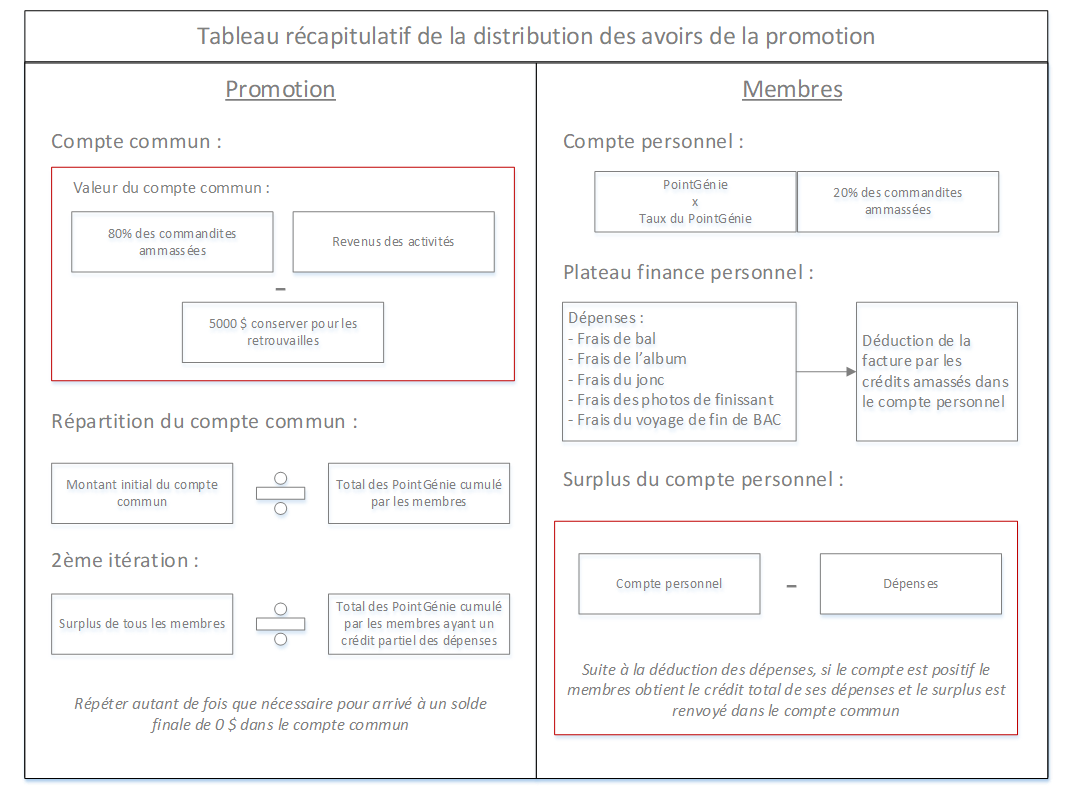
\includegraphics[width = 16cm]{Avoirs1.PNG}
\newpage
}
{\centering\section{ANNEXE C – Code Morin}}
\fbox{\parbox{\textwidth}{{\centering\textbf{Le Code Morin en bref}\par}
Voici  un  résumé  des  procédures  d’assemblées  délibérantes  du  code  Morin.  Ainsi,  vous  comprendrez de façon claire la procédure à respecter lors d’une assemblée générale et serez en mesure de mieux en comprendre le déroulement et la façon dont vous pouvez intervenir. Pour tout autre détail prière de consulter le code Morin.
}}
\begin{multicols}{2}
\noindent
\textbf{La présidence d'Assemblée}\\
Facilite le déroulement de la réunion. Procède à l'ouverture de la réunion puis la préside. Accorde le droit de parole et dirige l'Assemblée au  niveau des procédures et des discussions.  Rappelle à l'ordre tout membre qui ne respecte pas  l'ordre, les procédures et/ou le décorum.  Décide des points d'ordre et peut faire des sanctions publiques lorsqu'elles s'imposent.  Doit être impartiale sauf s'il y a égalité dans un vote; dans un tel cas, elle doit décider si la proposition est  acceptée ou non.

\bigskip
\noindent
\textbf{Ouverture de la réunion}\\
Le président d'Assemblée, appelle les membres à l'ordre, fait la lecture de l'ordre du jour puis demande le vote. Le secrétaire fait ensuite la lecture du procès verbal de la dernière réunion puis le-la président-e d'Assemblée demande le vote.\\
*À noter que l'ordre du jour et le procès verbal sont d'abord proposés et appuyés mais seulement adoptés après que les modifications nécessaires y aient été apportées (au besoin).\\
*Le procès verbal ne peut être adopté que par les membres présents lors de la réunion dont il traite.

\bigskip
\noindent
\textbf{Droit de parole}\\
Tout membre de l’assemblée a le droit de s'exprimer en réunion : il doit lever la main et attendre que le président d'Assemblée lui donne la parole. L'intervention doit être limitée au sujet débattu au moment.\\
*À noter que le président d'Assemblée a le droit de limiter la durée de même que le nombre 
d'interventions pour chaque sujet.

\bigskip
\noindent
\textbf{La proposition principale}\\
N'importe quel membre votant de l'assemblée peut formuler une proposition en autant que celle-
ci porte sur le point débattu à l'ordre du jour. Le « proposeur » doit attendre que le président d'Assemblée lui donne la parole, puis doit énoncer sa proposition comme suit : « Monsieur le président , je propose que... » La proposition doit ensuite être appuyée comme suit: « Monsieur le président , j'appuie. »\\
*À noter qu'une proposition est apportée lorsqu'on veut qu'une décision soit prise sur le sujet discuté.

\bigskip
\noindent
\textbf{L'amendement}\\
Sert à apporter une modification à la proposition principale. Doit porter sur la proposition débattue / doit être proposé et appuyé.\\
*À noter qu'un membre proposant un amendement doit en principe être d'accord avec la proposition et ne vouloir changer qu'un détail (le sens de la proposition doit demeurer le même).

\bigskip
\noindent
\textbf{Le sous-amendement}\\ 
C'est un amendement à un amendement qui a pour but de modifier un détail. Doit être proposé et appuyé.\\
*À noter qu'on peut seulement faire un (1) amendement et un (1) sous-amendement à la 
même proposition principale.\\
*Lorsqu'une proposition a reçu un amendement et un sous-amendement les discussions suivies 
du vote doivent se faire dans l'ordre suivant: le sous-amendement, l'amendement et terminer 
avec la proposition principale.
\end{multicols}
\newpage
\begin{multicols}{2}
\noindent
\textbf{Le vote}\\
A lieu à la fin d'un débat lorsque le président d'Assemblée pose officiellement la question débattue et demande ensuite le vote. Peut se faire à main levée ou par scrutin secret si un 
membre de l’assemblée le demande. (Tout membre votant peut l'exiger.)\\
*À noter qu'en général un vote requiert 50\% +1, sauf dans certains cas où il devra être 2/3, 3/4 ou encore unanime.\\ 
*Si le « proposeur » reprend la parole il conclut la discussion et l'Assemblée passe alors 
immédiatement au vote (sous la direction du président d'Assemblée).

\bigskip
\noindent
\textbf{Question préalable et / ou demande de vote}\\
Sert à mettre fin á tout débat lorsqu'un membre croit qu'il est temps de prendre une décision par rapport à un vote. Le membre doit demander la parole au président d'Assemblée puis poser la question préalable ou demander le vote. Lorsque cette demande est faite, le président exige (sans discussion) le vote de l'assemblée.\\
*À noter que la question préalable requiert les 2/3 de assemblée pour être adoptée.\\
*Si tel est le cas, seul le « proposeur » peut conclure la discussion et le vote s'en suivra. 

\bigskip
\noindent
\textbf{Proposition déposée sur le bureau}\\
Lorsque l'Assemblée a débattu un sujet, épuisé les idées et qu'aucune solution ne semble émerger de la discussion, un membre peut alors demander que la question soit déposée sur le bureau. La question est donc remise à plus tard et ce, jusqu'à ce que quelqu'un-une la ramène en discussion.\\
*À noter que cette proposition doit être proposée et appuyée sans discussion ou amendement et que le vote doit rallier la majorité simple de l'assemblée (50\% + 1).

\bigskip
\noindent
\textbf{Point d'ordre}\\
Utilisé lorsqu'un membre croit que les procédures ne sont pas respectées / pour énoncer une 
objection. Doit être formulé comme suit: « Monsieur le président, point d'ordre. »\\
*À noter que le président d'Assemblée prend la décision pour ou contre l'objection.

\bigskip
\noindent
\textbf{Point d'information}\\
Utilisé lorsqu'un membre ne comprend pas les procédures en rapport à une question concernant le point débattu. Peut se faire à n'importe quel moment de la réunion. Doit être formulé comme 
suit: « Monsieur le président, point d'information. »

\bigskip
\noindent
\textbf{Point de privilège}\\
Utilisé lorsqu'un membre croit que ses droits ne sont pas respectés et que le déroulement de la
réunion est incorrect. Peut se faire à n'importe quel moment de la réunion. Doit être formulé comme suit: « Monsieur le président, point de privilège. »

\bigskip
\noindent
\textbf{Déroulement typique d'une proposition venant de l’ assemblée}\\
Le « proposeur » présente sa motion lors du point à l'ordre du jour intitulé « propositions de l'Assemblée. » Un autre membre appuie la motion. La motion est remise par écrit au secrétaire d'Assemblée. Le « proposeur » ouvre le débat et explique sa motion (parle en premier). Il peut ensuite répondre à des questions lors du débat mais ne peut pas reprendre la parole sans quoi elle clôt le débat.  Après le temps prévu pour le débat, le président d'Assemblée demande le vote. La proposition est alors adoptée ou défaite.\\
\end{multicols}
\textit{* Le masculin est utilisé afin de faciliter la lecture du texte, il représente aussi la forme féminine.}
\newpage
%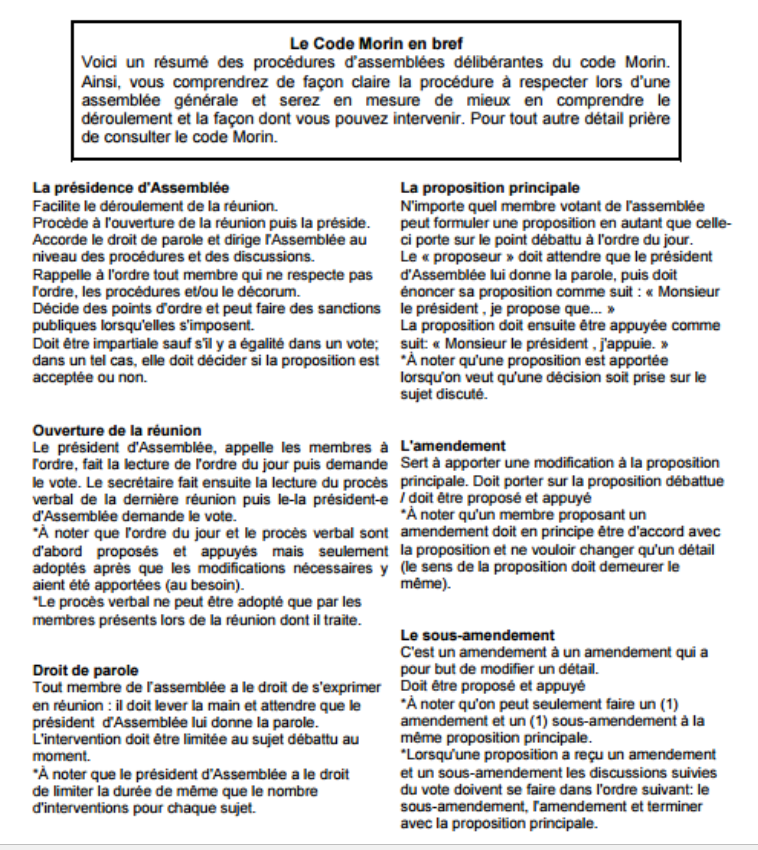
\includegraphics[width = 16cm]{Code1.PNG}
%\newpage
%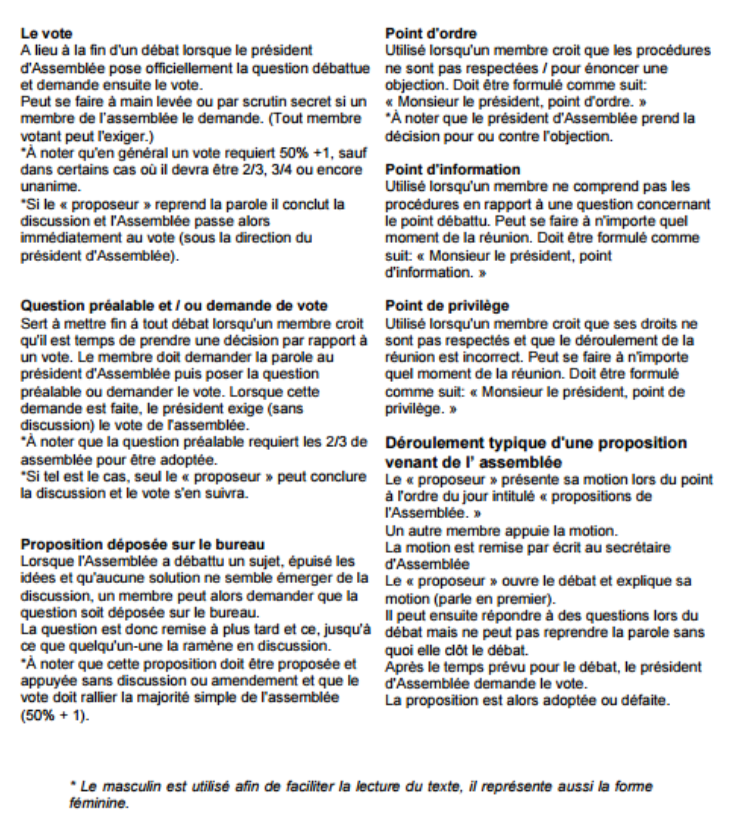
\includegraphics[width = 16cm]{Code2.PNG}
%\newpage
{\centering
\section{ANNEXE D – Règlement 50 de l’AGEG}
}
\makeatletter
\renewcommand\section{
	\@startsection{section}{1}{\z@}%
	{-3.5ex\@plus -1ex \@minus -.2ex}%
	{1.5ex \@plus .2ex}%
	{\normalfont\large\bfseries}*
}
\renewcommand\subsection{
	\@startsection{subsection}{2}{3.25ex}%
	{-1.625ex\@plus -1ex \@minus -.2ex}%
	{.75ex \@plus .2ex}%
	{\normalfont\normalsize\bfseries}*
}
\renewcommand\subsubsection{
	\@startsection{subsubsection}{3}{6.5ex}%
	{-1.625ex\@plus -1ex \@minus -.2ex}%
	{.75ex \@plus .2ex}%
	{\normalfont\normalsize\bfseries}*
}
\renewcommand\paragraph{\@startsection{paragraph}{4}{\z@}%
	{\z@}%3.25ex \@plus1ex \@minus.2ex}% beforeskip: Absolute value = skip to leave above the heading. If negative, then paragraph indent of text following heading is suppressed.
	{-1em}% afterskip : If positive, then skip to leave below heading, else negative of skip to leave to right of run-in heading.
	{\normalfont\normalsize\bfseries}* % style
}
\renewcommand\subparagraph{\@startsection{subparagraph}{5}{3.25ex}%
	{\z@}%
	{-1em}%
	{\normalfont\normalsize\bfseries}*
}

\newcounter{@agegPage}
\makeatother % Fin de l'edition des commandes
\preambule{Attendu que l'AGEG est responsable des groupes étudiants et promotions qu'elle supporte, notamment au niveau financier. Attendu que l'AGEG désire s'assurer de la pérennité des finances des groupes étudiants et promotions. Attendu que l'AGEG doit être en mesure de connaître l'ensemble des revenus et des dépenses des entités qui la constituent pour remplir ces exigences vis-a-vis les gouvernements fédéraux et provinciaux. Le présent règlement se veut une façon pour l'AGEG de s'assurer de la santé financière des groupes et d'assurer aux futurs étudiants d'hériter de gro aussi d'uniformiser les finances des différents groupes de l'AGEG pour permettre un meilleur suivi année après année, en plus de remplir ses obligations fiscales.}

\bigskip
\partie{Dispositions générales}
\article{Mission du réglements}
\alinea{Normativiser les finances des groupes étudiants et promotions pour en faciliter le suivi et s'assurer de la santé financière des groupes de l'AGEG.}
\alinea{Donner aux groupes les outils et la formation requis pour gérer leurs finances}
\alinea{Permettre à l'AGEG de remplir ses obligations fiscales par rapport aux groupes étudiants et promotions}

\article{Valeurs du règlement}
\valeurs{Ouverture}{Assurer que chaque groupe puisse établir ses états financiers selon sa propre réalité.}
{Engagement}{Garantir la pérennité financière des groupes en assurant une saine gestion financière.}
{Intégrité}{Faire preuve de dilligence dans la gestion financière des groupes étudiants et promotions.}
{Fraternité}{Permettre l'échange de connaissances sur la comptabilité entre les groupes étudiants et promotions et l'AGEG.}

\article{Rôles et pouvoirs}
\sousarticle{AGEG}  
\alinea{Elle met à disposition des groupes étudiant un accès pour un système comptable}
\alinea{Elle organise une formation pour les trésoriers des groupes sur l'utilisation du systême comptable.}
\alinea{Elle produit les déclarations fiscales reliées aux budgets des groupes techniques}
\alinea{Elle fait le paiment des taxes de ventes selon les déclarations dans le budget des groupes}
\alinea{Elle s'occuppe de l'archivage des documents financiers des groupes}
\alinea{Sous réception des avis de changement de signataires d'un groupe de l'AGEG, le CE émet une résolution et procède au changement.}

\sousarticle{VPAF de l'AGEG}
\alinea{En début de session, il met à jour le guide de gestion du budget des groupes et l'envoi aux groupes.}
\alinea{Il reçoit à chaque session le budget des groupes étudiants}
\alinea{Il s'assure que les budgets des groupes sont conformes aux normes}
\alinea{Il assure le remboursement du paiement des taxes de vente par les groupes}
\alinea{Sous résolution du CE, il change les signataires des groupes ayant leur compte de banque lié à celui de l'AGEG après présentation des nouveaux signataires}

\sousarticle{VPAX de l'AGEG}
\alinea{Il tient à jour la liste des trésoriers des groupes étudiants et promotions.}

\sousarticle{groupes étudiants et promotions}
\alinea{Il nomme un trésorier qui doit s'occuper de la comptabilité du groupe}
\alinea{Il s'assure que le trésorier remplit correctement les obligations financières du groupe}
\alinea{Il remplit son budget selon les normes établies par le guide de gestion du budget des groupes.}
\alinea{Il envoie son budget à chaque session aux VPAF de l'AGEG.}
\alinea{Il s'assure de conserver les documents financiers suivants pour une période de trois ans, après quoi, il sont remis à l'AGEG pour archivage:}
\sousalinea{Copie électronique des factures payées par le groupe}
\sousalinea{Copie électronique des chèques reçus par le groupe}
\sousalinea{Copie électronique des relevés de compte mensuels du groupe}
\alinea{Il rembourse l'AGEG pour le paiement des taxes de ventes}
\alinea{Il avertit l'AGEG pour une  modification aux signataires de son compte}

\article{Accès au système comptable}
\alinea{L'AGEG met a la disposition des groupes un accès utilisateur à un systême comptable.}
\alinea{L'AGEG conserve l'accès administrateur des groupes dans le systême comptable}

\article{Non-respect des normes}
\alinea{Un non-respect des normes par un groupe peut entraîner les conséquences suivantes:}
\sousalinea{Pour un groupe technique: réduction ou supression de la subvention de l'AGEG.}
\sousalinea{Pour une promotion: perte de la semaine de financement.}
\sousalinea{Pour les autres groupes: perte de l'accès au financement du fonds de la moisson et du fonds de la direction.}
\alinea{Le groupe est responsable de surveiller le travail de son trésorier, le groupe est responsable du non-respect des normes.}

\article{Trésorier des groupes étudiants et des promotions}
\alinea{Les groupes étudiants et les promotions doivent nommer un trésoier}
\alinea{Le trésorier doit s'assurer de suivre la formation sur la gestion du budget des groupes et des promotions}
\alinea{Il doit être signataire du compte du groupe}
\alinea{Le groupe doit indiquer le nom de son trésorier à l'AGEG.}

\article{Compte de banque de l'AGEG}
\alinea{Les groupes de l'AGEG sont obligés d'avoir leur compte de banque lié à celui de l'AGEG chez son fournisseur de service bancaire}
\alinea{L'AGEG doit offrir son entente de tarification aux comptes de banques liés au sien.}

\adoption{21 juillet 2015}{23 juillet 2015}
\end{document}